\documentclass[11pt,ignorenonframetext,]{beamer}
\setbeamertemplate{caption}[numbered]
\setbeamertemplate{caption label separator}{: }
\setbeamercolor{caption name}{fg=normal text.fg}
\beamertemplatenavigationsymbolsempty
\usepackage{lmodern}
\usepackage{amssymb,amsmath}
\usepackage{ifxetex,ifluatex}
\usepackage{fixltx2e} % provides \textsubscript
\ifnum 0\ifxetex 1\fi\ifluatex 1\fi=0 % if pdftex
  \usepackage[T1]{fontenc}
  \usepackage[utf8]{inputenc}
\else % if luatex or xelatex
  \ifxetex
    \usepackage{mathspec}
  \else
    \usepackage{fontspec}
  \fi
  \defaultfontfeatures{Ligatures=TeX,Scale=MatchLowercase}
\fi
\usetheme[]{metropolis}
% use upquote if available, for straight quotes in verbatim environments
\IfFileExists{upquote.sty}{\usepackage{upquote}}{}
% use microtype if available
\IfFileExists{microtype.sty}{%
\usepackage{microtype}
\UseMicrotypeSet[protrusion]{basicmath} % disable protrusion for tt fonts
}{}
\newif\ifbibliography
\hypersetup{
            pdftitle={Lecture 17},
            pdfauthor={Colin Rundel},
            pdfborder={0 0 0},
            breaklinks=true}
\urlstyle{same}  % don't use monospace font for urls
\usepackage{color}
\usepackage{fancyvrb}
\newcommand{\VerbBar}{|}
\newcommand{\VERB}{\Verb[commandchars=\\\{\}]}
\DefineVerbatimEnvironment{Highlighting}{Verbatim}{commandchars=\\\{\}}
% Add ',fontsize=\small' for more characters per line
\newenvironment{Shaded}{}{}
\newcommand{\KeywordTok}[1]{\textcolor[rgb]{0.00,0.44,0.13}{\textbf{#1}}}
\newcommand{\DataTypeTok}[1]{\textcolor[rgb]{0.56,0.13,0.00}{#1}}
\newcommand{\DecValTok}[1]{\textcolor[rgb]{0.25,0.63,0.44}{#1}}
\newcommand{\BaseNTok}[1]{\textcolor[rgb]{0.25,0.63,0.44}{#1}}
\newcommand{\FloatTok}[1]{\textcolor[rgb]{0.25,0.63,0.44}{#1}}
\newcommand{\ConstantTok}[1]{\textcolor[rgb]{0.53,0.00,0.00}{#1}}
\newcommand{\CharTok}[1]{\textcolor[rgb]{0.25,0.44,0.63}{#1}}
\newcommand{\SpecialCharTok}[1]{\textcolor[rgb]{0.25,0.44,0.63}{#1}}
\newcommand{\StringTok}[1]{\textcolor[rgb]{0.25,0.44,0.63}{#1}}
\newcommand{\VerbatimStringTok}[1]{\textcolor[rgb]{0.25,0.44,0.63}{#1}}
\newcommand{\SpecialStringTok}[1]{\textcolor[rgb]{0.73,0.40,0.53}{#1}}
\newcommand{\ImportTok}[1]{#1}
\newcommand{\CommentTok}[1]{\textcolor[rgb]{0.38,0.63,0.69}{\textit{#1}}}
\newcommand{\DocumentationTok}[1]{\textcolor[rgb]{0.73,0.13,0.13}{\textit{#1}}}
\newcommand{\AnnotationTok}[1]{\textcolor[rgb]{0.38,0.63,0.69}{\textbf{\textit{#1}}}}
\newcommand{\CommentVarTok}[1]{\textcolor[rgb]{0.38,0.63,0.69}{\textbf{\textit{#1}}}}
\newcommand{\OtherTok}[1]{\textcolor[rgb]{0.00,0.44,0.13}{#1}}
\newcommand{\FunctionTok}[1]{\textcolor[rgb]{0.02,0.16,0.49}{#1}}
\newcommand{\VariableTok}[1]{\textcolor[rgb]{0.10,0.09,0.49}{#1}}
\newcommand{\ControlFlowTok}[1]{\textcolor[rgb]{0.00,0.44,0.13}{\textbf{#1}}}
\newcommand{\OperatorTok}[1]{\textcolor[rgb]{0.40,0.40,0.40}{#1}}
\newcommand{\BuiltInTok}[1]{#1}
\newcommand{\ExtensionTok}[1]{#1}
\newcommand{\PreprocessorTok}[1]{\textcolor[rgb]{0.74,0.48,0.00}{#1}}
\newcommand{\AttributeTok}[1]{\textcolor[rgb]{0.49,0.56,0.16}{#1}}
\newcommand{\RegionMarkerTok}[1]{#1}
\newcommand{\InformationTok}[1]{\textcolor[rgb]{0.38,0.63,0.69}{\textbf{\textit{#1}}}}
\newcommand{\WarningTok}[1]{\textcolor[rgb]{0.38,0.63,0.69}{\textbf{\textit{#1}}}}
\newcommand{\AlertTok}[1]{\textcolor[rgb]{1.00,0.00,0.00}{\textbf{#1}}}
\newcommand{\ErrorTok}[1]{\textcolor[rgb]{1.00,0.00,0.00}{\textbf{#1}}}
\newcommand{\NormalTok}[1]{#1}

% Prevent slide breaks in the middle of a paragraph:
\widowpenalties 1 10000
\raggedbottom

\AtBeginPart{
  \let\insertpartnumber\relax
  \let\partname\relax
  \frame{\partpage}
}
\AtBeginSection{
  \ifbibliography
  \else
    \let\insertsectionnumber\relax
    \let\sectionname\relax
    \frame{\sectionpage}
  \fi
}
\AtBeginSubsection{
  \let\insertsubsectionnumber\relax
  \let\subsectionname\relax
  \frame{\subsectionpage}
}

\setlength{\parindent}{0pt}
\setlength{\parskip}{6pt plus 2pt minus 1pt}
\setlength{\emergencystretch}{3em}  % prevent overfull lines
\providecommand{\tightlist}{%
  \setlength{\itemsep}{0pt}\setlength{\parskip}{0pt}}
\setcounter{secnumdepth}{0}

\usepackage{geometry}
\usepackage{graphicx}
\usepackage{amssymb}
\usepackage{color}          	% gives color options
\usepackage{url}		% produces hyperlinks
\usepackage[english]{babel}
\usepackage{colortbl}	% allows for color usage in tables
\usepackage{multirow}	% allows for rows that span multiple rows in tables
\usepackage{xcolor}		% this package has a variety of color options
\usepackage{calc}
\usepackage{multicol}
\usepackage{wrapfig}
\usepackage{textcomp}
\usepackage{bm}
\usepackage{bbm}
\usepackage{setspace}
\usepackage{changepage}
\singlespacing

\usepackage{fontspec}
\newfontfamily\DejaSans{DejaVu Sans}

%%%%%%%%%%%%%%%%
% Small code output
%%%%%%%%%%%%%%%%

%% change fontsize of R code

\makeatletter
\@ifundefined{Shaded}{\newenvironment{Shaded}{}{}}{}
\makeatother


\let\oldShaded\Shaded
\let\endoldShaded\endShaded
\renewenvironment{Shaded}{\footnotesize\begin{spacing}{0.9}\oldShaded}{\endoldShaded\end{spacing}}

%% change fontsize of output
\let\oldverbatim\verbatim
\let\endoldverbatim\endverbatim
\renewenvironment{verbatim}{\footnotesize\begin{spacing}{0.9}\oldverbatim}{\endoldverbatim\end{spacing}}


\newcommand{\tinyoutput}{
  \renewenvironment{Shaded}{\tiny\begin{spacing}{0.9}\oldShaded}{\endoldShaded\end{spacing}}
  \renewenvironment{verbatim}{\tiny\begin{spacing}{0.9}\oldverbatim}{\endoldverbatim\end{spacing}}
}

\newcommand{\scriptoutput}{
  \renewenvironment{Shaded}{\scriptsize\begin{spacing}{0.9}\oldShaded}{\endoldShaded\end{spacing}}
  \renewenvironment{verbatim}{\scriptsize\begin{spacing}{0.9}\oldverbatim}{\endoldverbatim\end{spacing}}
}

\newcommand{\footnoteoutput}{
  \renewenvironment{Shaded}{\footnotesize\begin{spacing}{0.9}\oldShaded}{\endoldShaded\end{spacing}}
  \renewenvironment{verbatim}{\footnotesize\begin{spacing}{0.9}\oldverbatim}{\endoldverbatim\end{spacing}}
}

%\newcommand{\verbatimfont}[1]{\renewcommand{\verbatim@font}{\ttfamily#1}}


%%%%%%%%%%%%%%%%
% Custom Colors
%%%%%%%%%%%%%%%%

\xdefinecolor{oiBlue}{rgb}{0.15, 0.35, 0.55}
\xdefinecolor{gray}{rgb}{0.5, 0.5, 0.5}
\xdefinecolor{darkGray}{rgb}{0.3, 0.3, 0.3}
\xdefinecolor{darkerGray}{rgb}{0.2, 0.2, 0.2}
\xdefinecolor{rubineRed}{rgb}{0.89,0,0.30}
\xdefinecolor{linkCol}{rgb}{0.11,0.49,0.95}	
\xdefinecolor{irishGreen}{rgb}{0,0.60,0}	
\xdefinecolor{darkturquoise}{rgb}{0.44, 0.58, 0.86}
\definecolor{lightGreen}{rgb}{0.533,0.765,0.42}
%\xdefinecolor{hlblue}{rgb}{0.051,0.65,1}
\xdefinecolor{hlblue}{rgb}{ 0.055, 0.639, 0.831}
\definecolor{light}{rgb}{.337,.608,.741}
\definecolor{dark}{rgb}{.337,.608,.741}

\definecolor{cpink}{rgb}{0.93, 0.23, 0.51}

%%%%%%%%%%%%%%%%
% Custom Commands
%%%%%%%%%%%%%%%%

% text colors
\newcommand{\red}[1]{\textit{\textcolor{rubineRed}{#1}}}
\newcommand{\orange}[1]{\textit{\textcolor{orange}{#1}}}
\newcommand{\pink}[1]{\textit{\textcolor{rubineRed!90!white!50}{#1}}}
\newcommand{\green}[1]{\textit{\textcolor{irishGreen}{#1}}}
\newcommand{\blue}[1]{\textit{\textcolor{darkturquoise}{#1}}}
\newcommand{\light}[1]{\textcolor{light}{\textbf{#1}}}
\newcommand{\dark}[1]{\textcolor{dark}{#1}}
\newcommand{\gray}[1]{\textcolor{gray}{#1}}


% links: webURL, webLin, appLink
\newcommand{\webURL}[1]{\urlstyle{same}{\textit{\textcolor{linkCol}{\url{#1}}} }}
\newcommand{\webLink}[2]{\href{#1}{\textcolor{linkCol}{{#2}}}}
\newcommand{\appLink}[2]{\href{#1}{\textcolor{lightGreen!80!black!90}{{#2}}}}

% mail
\newcommand{\mail}[1]{\href{mailto:#1}{\textit{\textcolor{linkCol}{#1}}}}

% highlighting: hl, hlGr, mathhl
\newcommand{\hl}[1]{\textit{\textcolor{hlblue}{#1}}}
\newcommand{\hlGr}[1]{\textit{\textcolor{lightGreen}{#1}}}
\newcommand{\hlRd}[1]{\textit{\textcolor{rubineRed}{#1}}}
\newcommand{\mathhl}[1]{\textcolor{hlblue}{\ensuremath{#1}}}

% example
\newcommand{\ex}[1]{\textcolor{blue}{{{\small (#1)}}}}


\DeclareMathOperator*{\argmin}{arg\,min}
\DeclareMathOperator*{\argmax}{arg\,max}

\title{Lecture 17}
\subtitle{Spatial Data and Cartography (Part 2)}
\author{Colin Rundel}
\date{03/22/2017}

\begin{document}
\frame{\titlepage}

\section{Plotting}\label{plotting}

\begin{frame}[fragile,t]{Example Data - NC SIDS}

\scriptoutput

\begin{Shaded}
\begin{Highlighting}[]
\NormalTok{nc =}\StringTok{ }\KeywordTok{st_read}\NormalTok{(}\KeywordTok{system.file}\NormalTok{(}\StringTok{"shape/nc.shp"}\NormalTok{, }\DataTypeTok{package=}\StringTok{"sf"}\NormalTok{), }\DataTypeTok{quiet =} \OtherTok{TRUE}\NormalTok{) }\OperatorTok\StringTok{ }
\StringTok{  }\KeywordTok{select}\NormalTok{(}\OperatorTok{-}\NormalTok{(AREA}\OperatorTok{:}\NormalTok{CNTY_ID), }\OperatorTok{-}\NormalTok{(FIPS}\OperatorTok{:}\NormalTok{CRESS_ID))}

\KeywordTok{head}\NormalTok{(nc, }\DataTypeTok{n =} \DecValTok{10}\NormalTok{)}
\NormalTok{## Simple feature collection with 10 features and 7 fields}
\NormalTok{## geometry type:  MULTIPOLYGON}
\NormalTok{## dimension:      XY}
\NormalTok{## bbox:           xmin: -81.74107 ymin: 36.07282 xmax: -75.77316 ymax: 36.58965}
\NormalTok{## epsg (SRID):    4267}
\NormalTok{## proj4string:    +proj=longlat +datum=NAD27 +no_defs}
\NormalTok{##           NAME BIR74 SID74 NWBIR74 BIR79 SID79 NWBIR79}
\NormalTok{## 1         Ashe  1091     1      10  1364     0      19}
\NormalTok{## 2    Alleghany   487     0      10   542     3      12}
\NormalTok{## 3        Surry  3188     5     208  3616     6     260}
\NormalTok{## 4    Currituck   508     1     123   830     2     145}
\NormalTok{## 5  Northampton  1421     9    1066  1606     3    1197}
\NormalTok{## 6     Hertford  1452     7     954  1838     5    1237}
\NormalTok{## 7       Camden   286     0     115   350     2     139}
\NormalTok{## 8        Gates   420     0     254   594     2     371}
\NormalTok{## 9       Warren   968     4     748  1190     2     844}
\NormalTok{## 10      Stokes  1612     1     160  2038     5     176}
\NormalTok{##                          geometry}
\NormalTok{## 1  MULTIPOLYGON(((-81.47275543...}
\NormalTok{## 2  MULTIPOLYGON(((-81.23989105...}
\NormalTok{## 3  MULTIPOLYGON(((-80.45634460...}
\NormalTok{## 4  MULTIPOLYGON(((-76.00897216...}
\NormalTok{## 5  MULTIPOLYGON(((-77.21766662...}
\NormalTok{## 6  MULTIPOLYGON(((-76.74506378...}
\NormalTok{## 7  MULTIPOLYGON(((-76.00897216...}
\NormalTok{## 8  MULTIPOLYGON(((-76.56250762...}
\NormalTok{## 9  MULTIPOLYGON(((-78.30876159...}
\NormalTok{## 10 MULTIPOLYGON(((-80.02567291...}
\end{Highlighting}
\end{Shaded}

\end{frame}

\begin{frame}[fragile,t]{Base Plots}

\scriptoutput

\begin{Shaded}
\begin{Highlighting}[]
\KeywordTok{plot}\NormalTok{(nc)}
\end{Highlighting}
\end{Shaded}

\begin{center}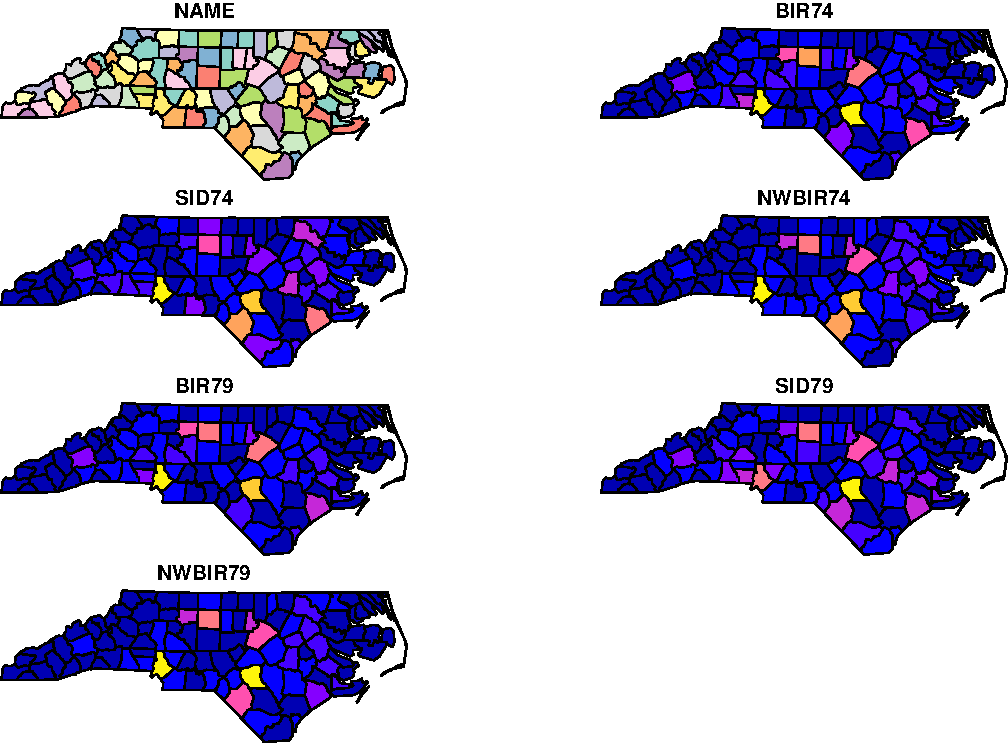
\includegraphics[width=0.8\textwidth]{Lec17_files/figure-beamer/unnamed-chunk-2-1} \end{center}

\end{frame}

\begin{frame}[fragile,t]{Geometry Plot}

\scriptoutput

\begin{Shaded}
\begin{Highlighting}[]
\KeywordTok{plot}\NormalTok{(}\KeywordTok{st_geometry}\NormalTok{(nc), }\DataTypeTok{axes=}\OtherTok{TRUE}\NormalTok{)}
\end{Highlighting}
\end{Shaded}

\begin{center}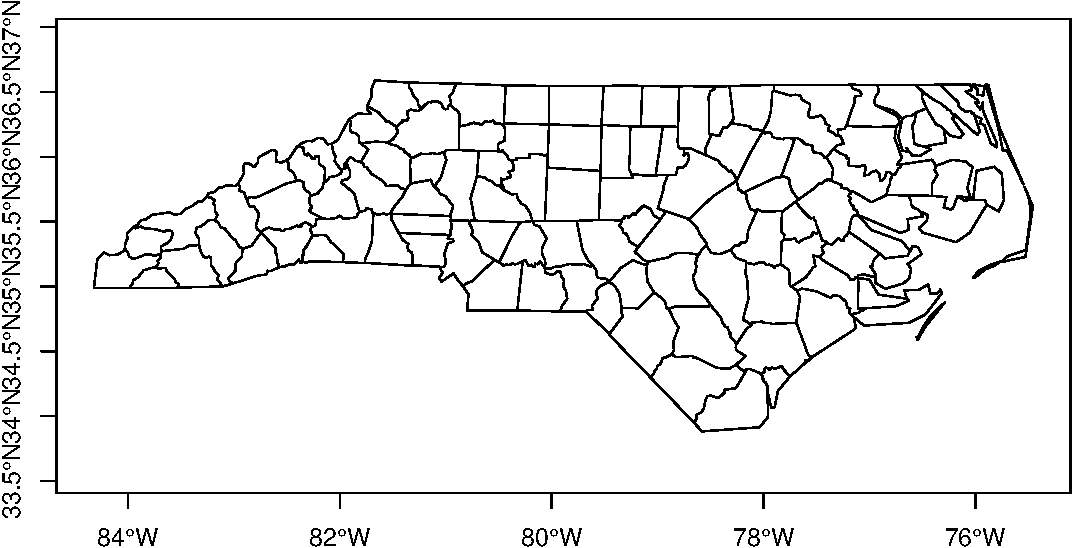
\includegraphics[width=0.95\textwidth]{Lec17_files/figure-beamer/unnamed-chunk-3-1} \end{center}

\end{frame}

\begin{frame}[fragile,t]{Graticules}

\scriptoutput

\begin{Shaded}
\begin{Highlighting}[]
\KeywordTok{plot}\NormalTok{(nc[,}\StringTok{"SID79"}\NormalTok{], }\DataTypeTok{graticule=}\KeywordTok{st_crs}\NormalTok{(nc), }\DataTypeTok{axes=}\OtherTok{TRUE}\NormalTok{, }\DataTypeTok{las=}\DecValTok{1}\NormalTok{)}
\end{Highlighting}
\end{Shaded}

\begin{center}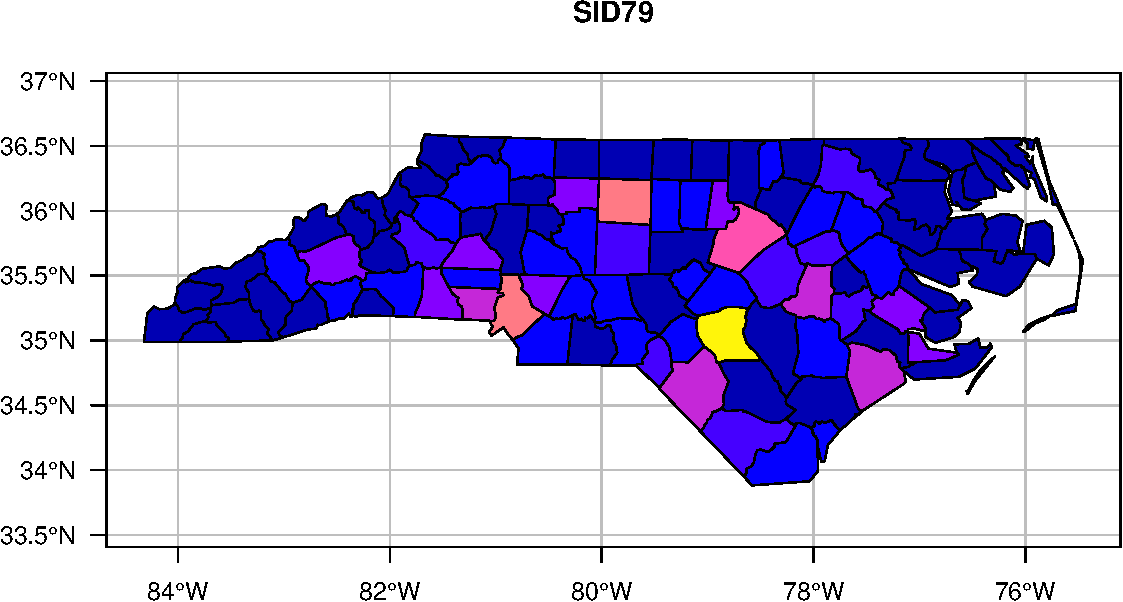
\includegraphics[width=0.95\textwidth]{Lec17_files/figure-beamer/unnamed-chunk-4-1} \end{center}

\end{frame}

\begin{frame}[fragile,t]{Graticules (EPSG:3631)}

\scriptoutput

\begin{Shaded}
\begin{Highlighting}[]
\KeywordTok{plot}\NormalTok{(}\KeywordTok{st_transform}\NormalTok{(nc[,}\StringTok{"SID79"}\NormalTok{], }\DecValTok{3631}\NormalTok{), }\DataTypeTok{graticule=}\KeywordTok{st_crs}\NormalTok{(nc), }\DataTypeTok{axes=}\OtherTok{TRUE}\NormalTok{, }\DataTypeTok{las=}\DecValTok{1}\NormalTok{)}
\end{Highlighting}
\end{Shaded}

\begin{center}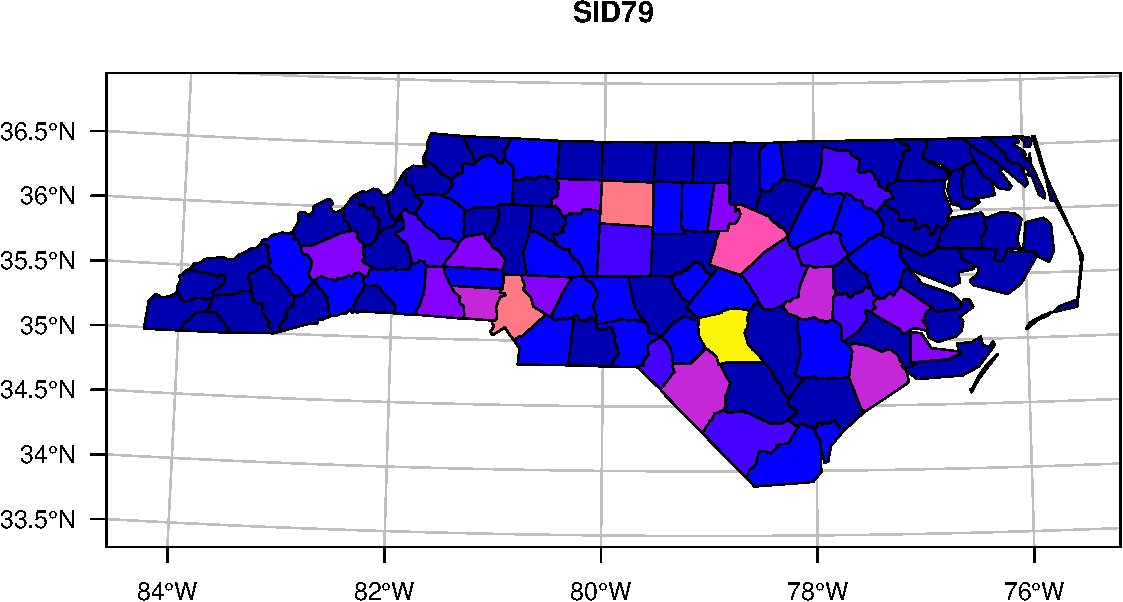
\includegraphics[width=0.95\textwidth]{Lec17_files/figure-beamer/unnamed-chunk-5-1} \end{center}

\end{frame}

\begin{frame}[fragile,t]{ggplot2 2.2.1.9 (dev)}

\scriptoutput

\begin{Shaded}
\begin{Highlighting}[]
\KeywordTok{ggplot}\NormalTok{(nc) }\OperatorTok{+}\StringTok{ }
\StringTok{  }\KeywordTok{geom_sf}\NormalTok{(}\KeywordTok{aes}\NormalTok{(}\DataTypeTok{fill=}\NormalTok{SID79 }\OperatorTok{/}\StringTok{ }\NormalTok{BIR79))}
\end{Highlighting}
\end{Shaded}

\begin{center}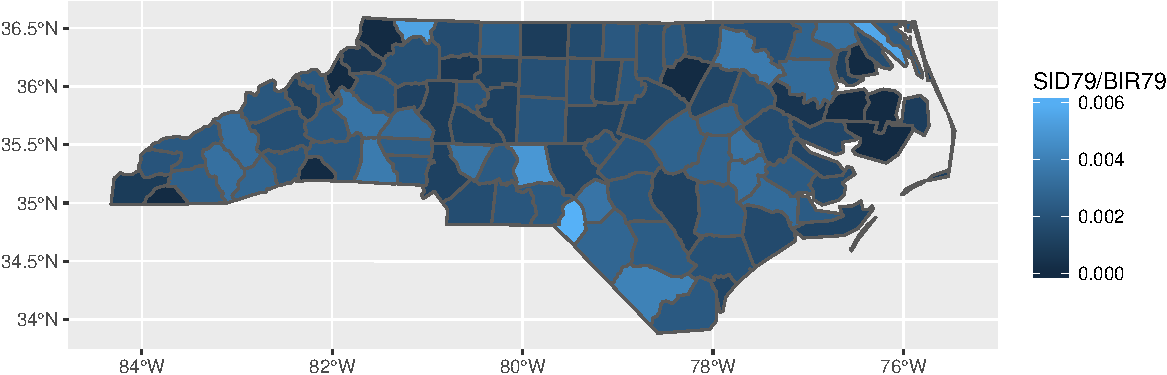
\includegraphics[width=0.95\textwidth]{Lec17_files/figure-beamer/unnamed-chunk-6-1} \end{center}

\end{frame}

\begin{frame}[fragile,t]{ggplot2 + projections}

\scriptoutput

\begin{Shaded}
\begin{Highlighting}[]
\KeywordTok{ggplot}\NormalTok{(}\KeywordTok{st_transform}\NormalTok{(nc, }\DecValTok{3631}\NormalTok{)) }\OperatorTok{+}\StringTok{ }
\StringTok{  }\KeywordTok{geom_sf}\NormalTok{(}\KeywordTok{aes}\NormalTok{(}\DataTypeTok{fill=}\NormalTok{SID79 }\OperatorTok{/}\StringTok{ }\NormalTok{BIR79))}
\end{Highlighting}
\end{Shaded}

\begin{center}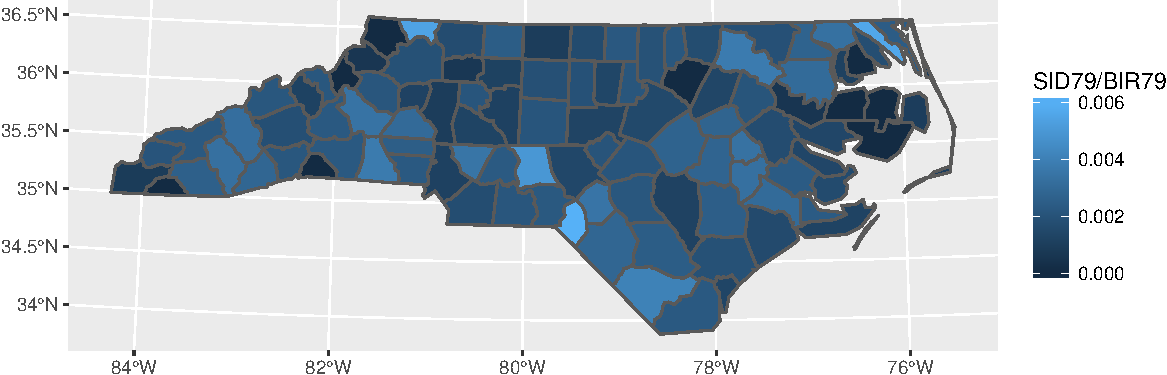
\includegraphics[width=0.95\textwidth]{Lec17_files/figure-beamer/unnamed-chunk-7-1} \end{center}

\end{frame}

\begin{frame}[fragile]{Example Data - Meuse}

\scriptoutput

\begin{Shaded}
\begin{Highlighting}[]
\KeywordTok{data}\NormalTok{(meuse, meuse.riv, }\DataTypeTok{package=}\StringTok{"sp"}\NormalTok{)}

\NormalTok{meuse =}\StringTok{ }\KeywordTok{st_as_sf}\NormalTok{(meuse, }\DataTypeTok{coords=}\KeywordTok{c}\NormalTok{(}\StringTok{"x"}\NormalTok{, }\StringTok{"y"}\NormalTok{), }\DataTypeTok{crs=}\DecValTok{28992}\NormalTok{)}
\NormalTok{meuse_riv =}\StringTok{ }\KeywordTok{st_polygon}\NormalTok{(}\KeywordTok{list}\NormalTok{(meuse.riv)) }\OperatorTok\StringTok{ }\KeywordTok{st_sfc}\NormalTok{() }\OperatorTok\StringTok{ }\KeywordTok{st_set_crs}\NormalTok{(}\DecValTok{28992}\NormalTok{)}

\NormalTok{meuse}
\NormalTok{## Simple feature collection with 155 features and 12 fields}
\NormalTok{## geometry type:  POINT}
\NormalTok{## dimension:      XY}
\NormalTok{## bbox:           xmin: 178605 ymin: 329714 xmax: 181390 ymax: 333611}
\NormalTok{## epsg (SRID):    28992}
\NormalTok{## proj4string:    +proj=sterea +lat_0=52.15616055555555 +lon_0=5.38763888888889 +k=0.9999079 +x_0=155000 +y_0=463000 +ellps=bessel +towgs84=565.4171,50.3319,465.5524,-0.398957,0.343988,-1.87740,4.0725 +units=m +no_defs}
\NormalTok{## First 20 features:}
\NormalTok{##    cadmium copper lead zinc  elev       dist   om ffreq soil lime}
\NormalTok{## 1     11.7     85  299 1022 7.909 0.00135803 13.6     1    1    1}
\NormalTok{## 2      8.6     81  277 1141 6.983 0.01222430 14.0     1    1    1}
\NormalTok{## 3      6.5     68  199  640 7.800 0.10302900 13.0     1    1    1}
\NormalTok{## 4      2.6     81  116  257 7.655 0.19009400  8.0     1    2    0}
\NormalTok{## 5      2.8     48  117  269 7.480 0.27709000  8.7     1    2    0}
\NormalTok{## 6      3.0     61  137  281 7.791 0.36406700  7.8     1    2    0}
\NormalTok{## 7      3.2     31  132  346 8.217 0.19009400  9.2     1    2    0}
\NormalTok{## 8      2.8     29  150  406 8.490 0.09215160  9.5     1    1    0}
\NormalTok{## 9      2.4     37  133  347 8.668 0.18461400 10.6     1    1    0}
\NormalTok{## 10     1.6     24   80  183 9.049 0.30970200  6.3     1    2    0}
\NormalTok{## 11     1.4     25   86  189 9.015 0.31511600  6.4     1    2    0}
\NormalTok{## 12     1.8     25   97  251 9.073 0.22812300  9.0     1    1    0}
\NormalTok{## 13    11.2     93  285 1096 7.320 0.00000000 15.4     1    1    1}
\NormalTok{## 14     2.5     31  183  504 8.815 0.11393200  8.4     1    1    0}
\NormalTok{## 15     2.0     27  130  326 8.937 0.16833600  9.1     1    1    0}
\NormalTok{## 16     9.5     86  240 1032 7.702 0.00000000 16.2     1    1    1}
\NormalTok{## 17     7.0     74  133  606 7.160 0.01222430 16.0     1    1    1}
\NormalTok{## 18     7.1     69  148  711 7.100 0.01222430 16.0     1    1    1}
\NormalTok{## 19     8.7     69  207  735 7.020 0.00000000 13.7     1    1    1}
\NormalTok{## 20    12.9     95  284 1052 6.860 0.00000000 14.8     1    1    1}
\NormalTok{##    landuse dist.m             geometry}
\NormalTok{## 1       Ah     50 POINT(181072 333611)}
\NormalTok{## 2       Ah     30 POINT(181025 333558)}
\NormalTok{## 3       Ah    150 POINT(181165 333537)}
\NormalTok{## 4       Ga    270 POINT(181298 333484)}
\NormalTok{## 5       Ah    380 POINT(181307 333330)}
\NormalTok{## 6       Ga    470 POINT(181390 333260)}
\NormalTok{## 7       Ah    240 POINT(181165 333370)}
\NormalTok{## 8       Ab    120 POINT(181027 333363)}
\NormalTok{## 9       Ab    240 POINT(181060 333231)}
\NormalTok{## 10       W    420 POINT(181232 333168)}
\NormalTok{## 11      Fh    400 POINT(181191 333115)}
\NormalTok{## 12      Ag    300 POINT(181032 333031)}
\NormalTok{## 13       W     20 POINT(180874 333339)}
\NormalTok{## 14      Ah    130 POINT(180969 333252)}
\NormalTok{## 15      Ah    220 POINT(181011 333161)}
\NormalTok{## 16       W     10 POINT(180830 333246)}
\NormalTok{## 17       W     10 POINT(180763 333104)}
\NormalTok{## 18       W     10 POINT(180694 332972)}
\NormalTok{## 19       W     10 POINT(180625 332847)}
\NormalTok{## 20    <NA>     10 POINT(180555 332707)}
\end{Highlighting}
\end{Shaded}

\end{frame}

\begin{frame}[fragile,t]{Meuse}

\scriptoutput

\begin{Shaded}
\begin{Highlighting}[]
\KeywordTok{plot}\NormalTok{(meuse, }\DataTypeTok{pch=}\DecValTok{16}\NormalTok{)}
\end{Highlighting}
\end{Shaded}

\begin{center}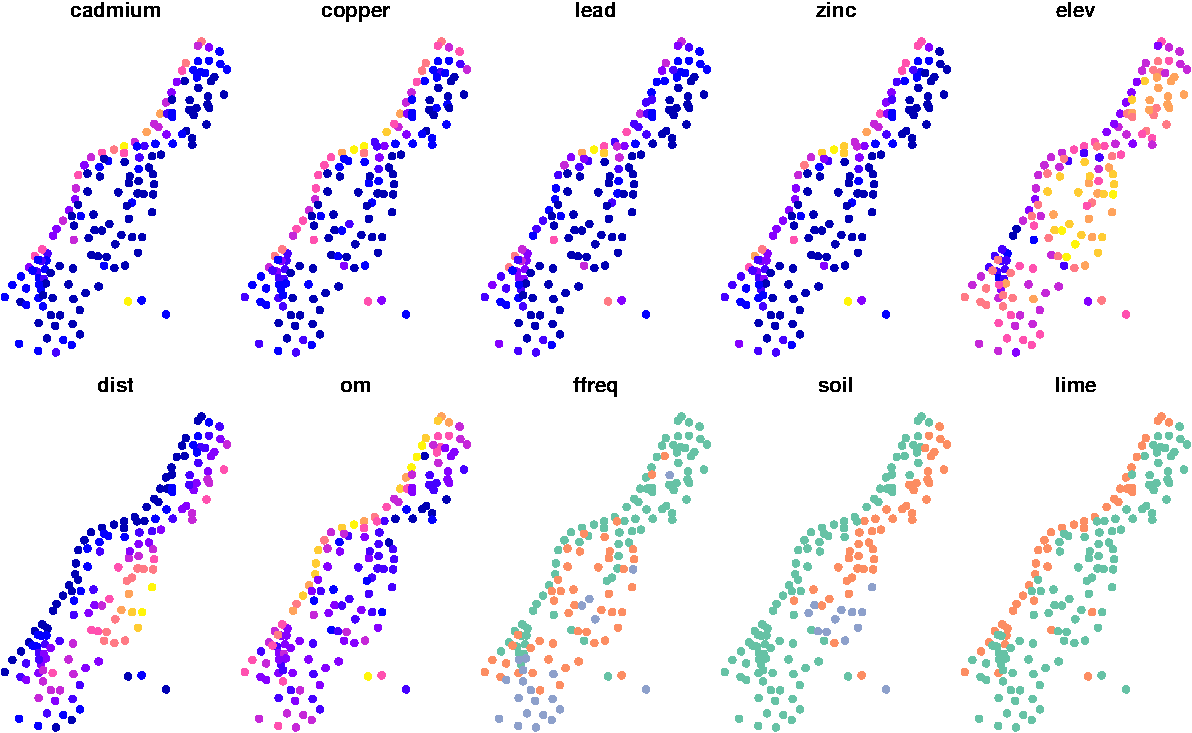
\includegraphics[width=0.95\textwidth]{Lec17_files/figure-beamer/unnamed-chunk-9-1} \end{center}

\end{frame}

\begin{frame}[fragile,t]{Layering plots}

\scriptoutput

\begin{Shaded}
\begin{Highlighting}[]
\KeywordTok{plot}\NormalTok{(meuse[,}\StringTok{"lead"}\NormalTok{], }\DataTypeTok{pch=}\DecValTok{16}\NormalTok{, }\DataTypeTok{axes=}\OtherTok{TRUE}\NormalTok{)}
\KeywordTok{plot}\NormalTok{(meuse_riv, }\DataTypeTok{col=}\KeywordTok{adjustcolor}\NormalTok{(}\StringTok{"lightblue"}\NormalTok{, }\DataTypeTok{alpha.f=}\FloatTok{0.5}\NormalTok{), }\DataTypeTok{add=}\OtherTok{TRUE}\NormalTok{, }\DataTypeTok{border =} \OtherTok{NA}\NormalTok{)}
\end{Highlighting}
\end{Shaded}

\begin{center}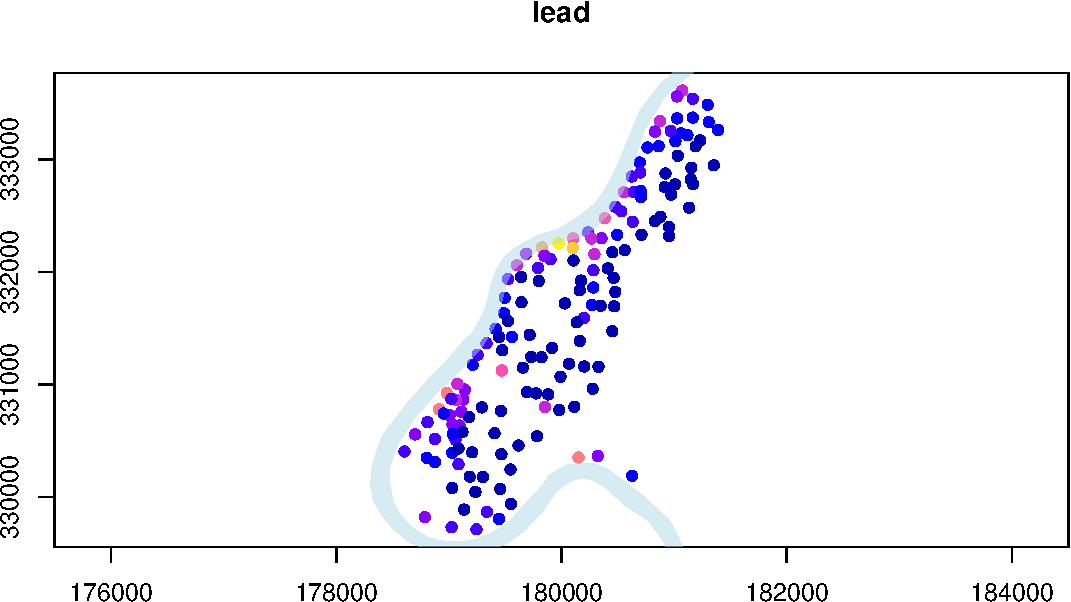
\includegraphics[width=0.95\textwidth]{Lec17_files/figure-beamer/unnamed-chunk-10-1} \end{center}

\end{frame}

\begin{frame}[fragile,t]{Layering plots (oops)}

\scriptoutput

\begin{Shaded}
\begin{Highlighting}[]
\KeywordTok{plot}\NormalTok{(meuse, }\DataTypeTok{pch=}\DecValTok{16}\NormalTok{)}
\KeywordTok{plot}\NormalTok{(meuse_riv, }\DataTypeTok{col=}\KeywordTok{adjustcolor}\NormalTok{(}\StringTok{"lightblue"}\NormalTok{, }\DataTypeTok{alpha.f=}\FloatTok{0.5}\NormalTok{), }\DataTypeTok{add=}\OtherTok{TRUE}\NormalTok{, }\DataTypeTok{border =} \OtherTok{NA}\NormalTok{)}
\end{Highlighting}
\end{Shaded}

\begin{center}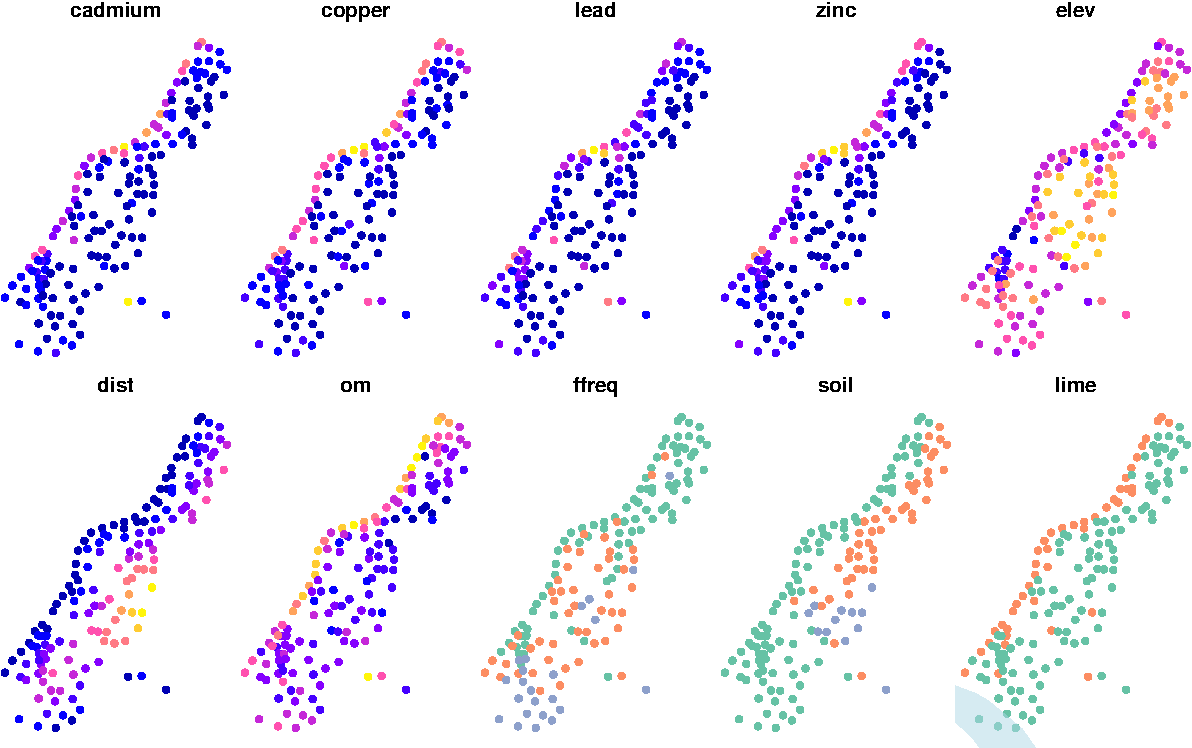
\includegraphics[width=0.95\textwidth]{Lec17_files/figure-beamer/unnamed-chunk-11-1} \end{center}

\end{frame}

\begin{frame}[fragile,t]{ggplot2}

\scriptoutput

\begin{Shaded}
\begin{Highlighting}[]
\KeywordTok{ggplot}\NormalTok{() }\OperatorTok{+}
\StringTok{  }\KeywordTok{geom_sf}\NormalTok{(}\DataTypeTok{data=}\KeywordTok{st_sf}\NormalTok{(meuse_riv), }\DataTypeTok{fill=}\StringTok{"lightblue"}\NormalTok{, }\DataTypeTok{color=}\OtherTok{NA}\NormalTok{) }\OperatorTok{+}
\StringTok{  }\KeywordTok{geom_sf}\NormalTok{(}\DataTypeTok{data=}\NormalTok{meuse, }\KeywordTok{aes}\NormalTok{(}\DataTypeTok{color=}\NormalTok{lead), }\DataTypeTok{size=}\DecValTok{1}\NormalTok{)}
\end{Highlighting}
\end{Shaded}

\begin{center}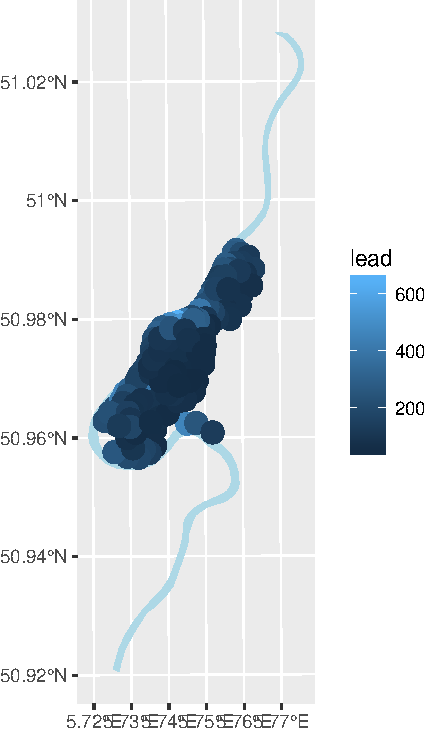
\includegraphics[width=0.33\textwidth]{Lec17_files/figure-beamer/unnamed-chunk-12-1} \end{center}

\end{frame}

\begin{frame}[fragile,t]{ggplot2 - axis limits}

\scriptoutput

\begin{Shaded}
\begin{Highlighting}[]
\KeywordTok{ggplot}\NormalTok{() }\OperatorTok{+}
\StringTok{  }\KeywordTok{geom_sf}\NormalTok{(}\DataTypeTok{data=}\KeywordTok{st_sf}\NormalTok{(meuse_riv), }\DataTypeTok{fill=}\StringTok{"lightblue"}\NormalTok{, }\DataTypeTok{color=}\OtherTok{NA}\NormalTok{) }\OperatorTok{+}
\StringTok{  }\KeywordTok{geom_sf}\NormalTok{(}\DataTypeTok{data=}\NormalTok{meuse, }\KeywordTok{aes}\NormalTok{(}\DataTypeTok{color=}\NormalTok{lead), }\DataTypeTok{size=}\FloatTok{0.1}\NormalTok{) }\OperatorTok{+}
\StringTok{  }\KeywordTok{ylim}\NormalTok{(}\DecValTok{329714}\NormalTok{, }\DecValTok{333611}\NormalTok{)}
\end{Highlighting}
\end{Shaded}

\begin{center}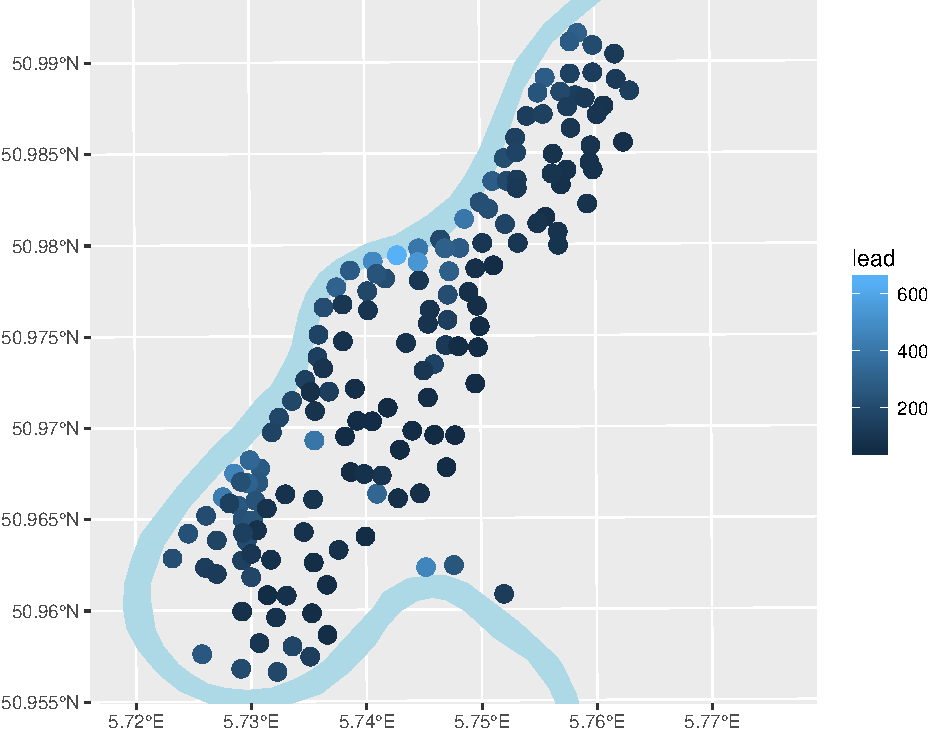
\includegraphics[width=0.65\textwidth]{Lec17_files/figure-beamer/unnamed-chunk-13-1} \end{center}

\end{frame}

\begin{frame}[fragile,t]{ggplot2 - bounding box}

\scriptoutput

\begin{Shaded}
\begin{Highlighting}[]
\KeywordTok{ggplot}\NormalTok{() }\OperatorTok{+}
\StringTok{  }\KeywordTok{geom_sf}\NormalTok{(}\DataTypeTok{data=}\KeywordTok{st_sf}\NormalTok{(meuse_riv), }\DataTypeTok{fill=}\StringTok{"lightblue"}\NormalTok{, }\DataTypeTok{color=}\OtherTok{NA}\NormalTok{) }\OperatorTok{+}
\StringTok{  }\KeywordTok{geom_sf}\NormalTok{(}\DataTypeTok{data=}\NormalTok{meuse, }\KeywordTok{aes}\NormalTok{(}\DataTypeTok{color=}\NormalTok{lead), }\DataTypeTok{size=}\FloatTok{0.1}\NormalTok{) }\OperatorTok{+}
\StringTok{  }\KeywordTok{ylim}\NormalTok{(}\KeywordTok{st_bbox}\NormalTok{(meuse)[}\StringTok{"ymin"}\NormalTok{], }\KeywordTok{st_bbox}\NormalTok{(meuse)[}\StringTok{"ymax"}\NormalTok{])}
\end{Highlighting}
\end{Shaded}

\begin{center}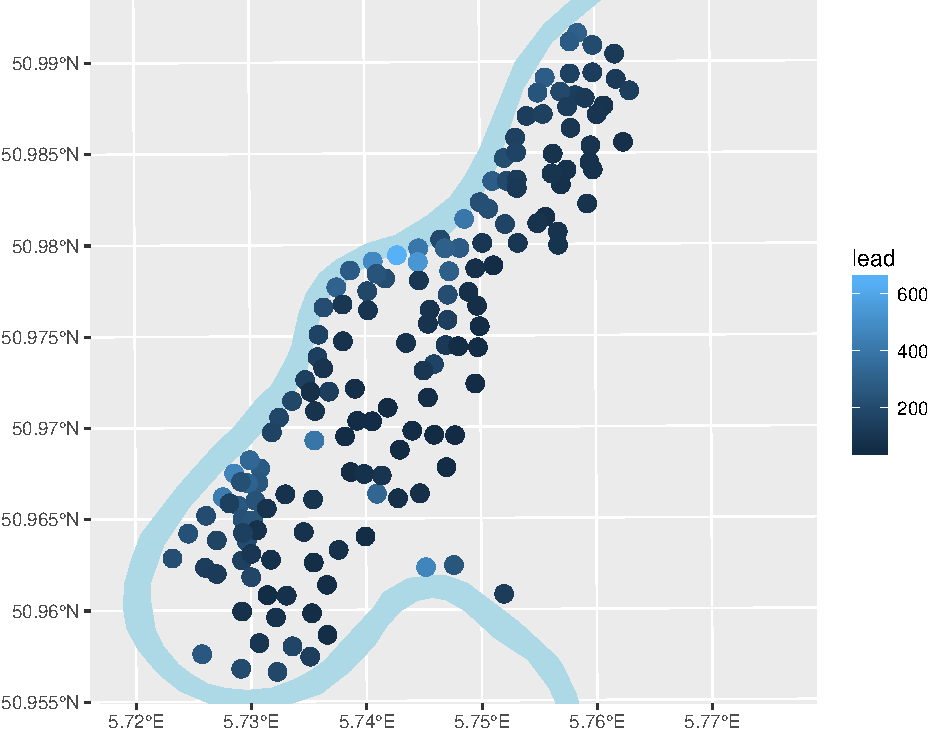
\includegraphics[width=0.65\textwidth]{Lec17_files/figure-beamer/unnamed-chunk-14-1} \end{center}

\end{frame}

\section{Geometry Manipulation}\label{geometry-manipulation}

\begin{frame}[fragile,t]{Casting}

\scriptoutput

\begin{Shaded}
\begin{Highlighting}[]
\NormalTok{nc_pts =}\StringTok{ }\KeywordTok{st_cast}\NormalTok{(nc, }\StringTok{"MULTIPOINT"}\NormalTok{)}

\NormalTok{nc_pts}
\NormalTok{## Simple feature collection with 100 features and 7 fields}
\NormalTok{## geometry type:  MULTIPOINT}
\NormalTok{## dimension:      XY}
\NormalTok{## bbox:           xmin: -84.32385 ymin: 33.88199 xmax: -75.45698 ymax: 36.58965}
\NormalTok{## epsg (SRID):    4267}
\NormalTok{## proj4string:    +proj=longlat +datum=NAD27 +no_defs}
\NormalTok{## First 20 features:}
\NormalTok{##           NAME BIR74 SID74 NWBIR74 BIR79 SID79 NWBIR79}
\NormalTok{## 1         Ashe  1091     1      10  1364     0      19}
\NormalTok{## 2    Alleghany   487     0      10   542     3      12}
\NormalTok{## 3        Surry  3188     5     208  3616     6     260}
\NormalTok{## 4    Currituck   508     1     123   830     2     145}
\NormalTok{## 5  Northampton  1421     9    1066  1606     3    1197}
\NormalTok{## 6     Hertford  1452     7     954  1838     5    1237}
\NormalTok{## 7       Camden   286     0     115   350     2     139}
\NormalTok{## 8        Gates   420     0     254   594     2     371}
\NormalTok{## 9       Warren   968     4     748  1190     2     844}
\NormalTok{## 10      Stokes  1612     1     160  2038     5     176}
\NormalTok{## 11     Caswell  1035     2     550  1253     2     597}
\NormalTok{## 12  Rockingham  4449    16    1243  5386     5    1369}
\NormalTok{## 13   Granville  1671     4     930  2074     4    1058}
\NormalTok{## 14      Person  1556     4     613  1790     4     650}
\NormalTok{## 15       Vance  2180     4    1179  2753     6    1492}
\NormalTok{## 16     Halifax  3608    18    2365  4463    17    2980}
\NormalTok{## 17  Pasquotank  1638     3     622  2275     4     933}
\NormalTok{## 18      Wilkes  3146     4     200  3725     7     222}
\NormalTok{## 19     Watauga  1323     1      17  1775     1      33}
\NormalTok{## 20  Perquimans   484     1     230   676     0     310}
\NormalTok{##                          geometry}
\NormalTok{## 1  MULTIPOINT(-81.472755432128...}
\NormalTok{## 2  MULTIPOINT(-81.239891052246...}
\NormalTok{## 3  MULTIPOINT(-80.456344604492...}
\NormalTok{## 4  MULTIPOINT(-76.008972167968...}
\NormalTok{## 5  MULTIPOINT(-77.217666625976...}
\NormalTok{## 6  MULTIPOINT(-76.745063781738...}
\NormalTok{## 7  MULTIPOINT(-76.008972167968...}
\NormalTok{## 8  MULTIPOINT(-76.562507629394...}
\NormalTok{## 9  MULTIPOINT(-78.308761596679...}
\NormalTok{## 10 MULTIPOINT(-80.025672912597...}
\NormalTok{## 11 MULTIPOINT(-79.530509948730...}
\NormalTok{## 12 MULTIPOINT(-79.530509948730...}
\NormalTok{## 13 MULTIPOINT(-78.749122619628...}
\NormalTok{## 14 MULTIPOINT(-78.806800842285...}
\NormalTok{## 15 MULTIPOINT(-78.492523193359...}
\NormalTok{## 16 MULTIPOINT(-77.332206726074...}
\NormalTok{## 17 MULTIPOINT(-76.298927307128...}
\NormalTok{## 18 MULTIPOINT(-81.020568847656...}
\NormalTok{## 19 MULTIPOINT(-81.806221008300...}
\NormalTok{## 20 MULTIPOINT(-76.480529785156...}
\end{Highlighting}
\end{Shaded}

\end{frame}

\begin{frame}[fragile,t]{}

\scriptoutput

\begin{Shaded}
\begin{Highlighting}[]
\KeywordTok{plot}\NormalTok{(}\KeywordTok{st_geometry}\NormalTok{(nc), }\DataTypeTok{border=}\StringTok{'grey'}\NormalTok{)}
\KeywordTok{plot}\NormalTok{(}\KeywordTok{st_geometry}\NormalTok{(nc_pts), }\DataTypeTok{pch=}\DecValTok{16}\NormalTok{, }\DataTypeTok{cex=}\FloatTok{0.5}\NormalTok{, }\DataTypeTok{add=}\OtherTok{TRUE}\NormalTok{)}
\end{Highlighting}
\end{Shaded}

\begin{center}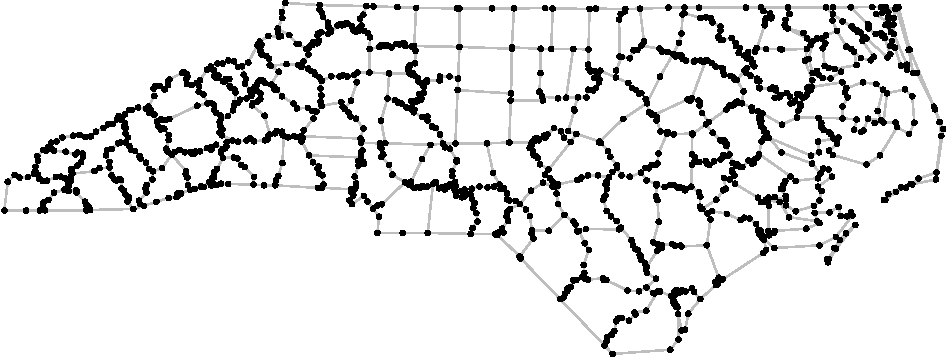
\includegraphics[width=0.95\textwidth]{Lec17_files/figure-beamer/unnamed-chunk-16-1} \end{center}

\end{frame}

\begin{frame}[fragile,t]{Casting - POINT}

\scriptoutput

\begin{Shaded}
\begin{Highlighting}[]
\KeywordTok{st_cast}\NormalTok{(nc, }\StringTok{"POINT"}\NormalTok{)}
\NormalTok{## Simple feature collection with 2529 features and 7 fields}
\NormalTok{## geometry type:  POINT}
\NormalTok{## dimension:      XY}
\NormalTok{## bbox:           xmin: -84.32385 ymin: 33.88199 xmax: -75.45698 ymax: 36.58965}
\NormalTok{## epsg (SRID):    4267}
\NormalTok{## proj4string:    +proj=longlat +datum=NAD27 +no_defs}
\NormalTok{## First 20 features:}
\NormalTok{##    NAME BIR74 SID74 NWBIR74 BIR79 SID79 NWBIR79}
\NormalTok{## 1  Ashe  1091     1      10  1364     0      19}
\NormalTok{## 2  Ashe  1091     1      10  1364     0      19}
\NormalTok{## 3  Ashe  1091     1      10  1364     0      19}
\NormalTok{## 4  Ashe  1091     1      10  1364     0      19}
\NormalTok{## 5  Ashe  1091     1      10  1364     0      19}
\NormalTok{## 6  Ashe  1091     1      10  1364     0      19}
\NormalTok{## 7  Ashe  1091     1      10  1364     0      19}
\NormalTok{## 8  Ashe  1091     1      10  1364     0      19}
\NormalTok{## 9  Ashe  1091     1      10  1364     0      19}
\NormalTok{## 10 Ashe  1091     1      10  1364     0      19}
\NormalTok{## 11 Ashe  1091     1      10  1364     0      19}
\NormalTok{## 12 Ashe  1091     1      10  1364     0      19}
\NormalTok{## 13 Ashe  1091     1      10  1364     0      19}
\NormalTok{## 14 Ashe  1091     1      10  1364     0      19}
\NormalTok{## 15 Ashe  1091     1      10  1364     0      19}
\NormalTok{## 16 Ashe  1091     1      10  1364     0      19}
\NormalTok{## 17 Ashe  1091     1      10  1364     0      19}
\NormalTok{## 18 Ashe  1091     1      10  1364     0      19}
\NormalTok{## 19 Ashe  1091     1      10  1364     0      19}
\NormalTok{## 20 Ashe  1091     1      10  1364     0      19}
\NormalTok{##                          geometry}
\NormalTok{## 1  POINT(-81.4727554321289 36....}
\NormalTok{## 2  POINT(-81.5408401489258 36....}
\NormalTok{## 3  POINT(-81.5619812011719 36....}
\NormalTok{## 4  POINT(-81.6330642700195 36....}
\NormalTok{## 5  POINT(-81.7410736083984 36....}
\NormalTok{## 6  POINT(-81.6982803344727 36....}
\NormalTok{## 7  POINT(-81.7027969360352 36....}
\NormalTok{## 8  POINT(-81.6699981689453 36....}
\NormalTok{## 9  POINT(-81.3452987670898 36....}
\NormalTok{## 10 POINT(-81.347541809082 36.5...}
\NormalTok{## 11 POINT(-81.3247756958008 36....}
\NormalTok{## 12 POINT(-81.3133239746094 36....}
\NormalTok{## 13 POINT(-81.2662353515625 36....}
\NormalTok{## 14 POINT(-81.2628402709961 36....}
\NormalTok{## 15 POINT(-81.2406921386719 36....}
\NormalTok{## 16 POINT(-81.2398910522461 36....}
\NormalTok{## 17 POINT(-81.2642440795898 36....}
\NormalTok{## 18 POINT(-81.3289947509766 36....}
\NormalTok{## 19 POINT(-81.3613739013672 36....}
\NormalTok{## 20 POINT(-81.3656921386719 36....}
\end{Highlighting}
\end{Shaded}

\end{frame}

\begin{frame}[fragile,t]{Casting - LINESTRING}

\scriptoutput

\begin{Shaded}
\begin{Highlighting}[]
\KeywordTok{st_cast}\NormalTok{(nc, }\StringTok{"LINESTRING"}\NormalTok{)}
\NormalTok{## Simple feature collection with 100 features and 7 fields}
\NormalTok{## geometry type:  LINESTRING}
\NormalTok{## dimension:      XY}
\NormalTok{## bbox:           xmin: -84.32385 ymin: 33.88199 xmax: -75.45698 ymax: 36.58965}
\NormalTok{## epsg (SRID):    4267}
\NormalTok{## proj4string:    +proj=longlat +datum=NAD27 +no_defs}
\NormalTok{## First 20 features:}
\NormalTok{##           NAME BIR74 SID74 NWBIR74 BIR79 SID79 NWBIR79}
\NormalTok{## 1         Ashe  1091     1      10  1364     0      19}
\NormalTok{## 2    Alleghany   487     0      10   542     3      12}
\NormalTok{## 3        Surry  3188     5     208  3616     6     260}
\NormalTok{## 4    Currituck   508     1     123   830     2     145}
\NormalTok{## 5  Northampton  1421     9    1066  1606     3    1197}
\NormalTok{## 6     Hertford  1452     7     954  1838     5    1237}
\NormalTok{## 7       Camden   286     0     115   350     2     139}
\NormalTok{## 8        Gates   420     0     254   594     2     371}
\NormalTok{## 9       Warren   968     4     748  1190     2     844}
\NormalTok{## 10      Stokes  1612     1     160  2038     5     176}
\NormalTok{## 11     Caswell  1035     2     550  1253     2     597}
\NormalTok{## 12  Rockingham  4449    16    1243  5386     5    1369}
\NormalTok{## 13   Granville  1671     4     930  2074     4    1058}
\NormalTok{## 14      Person  1556     4     613  1790     4     650}
\NormalTok{## 15       Vance  2180     4    1179  2753     6    1492}
\NormalTok{## 16     Halifax  3608    18    2365  4463    17    2980}
\NormalTok{## 17  Pasquotank  1638     3     622  2275     4     933}
\NormalTok{## 18      Wilkes  3146     4     200  3725     7     222}
\NormalTok{## 19     Watauga  1323     1      17  1775     1      33}
\NormalTok{## 20  Perquimans   484     1     230   676     0     310}
\NormalTok{##                          geometry}
\NormalTok{## 1  LINESTRING(-81.472755432128...}
\NormalTok{## 2  LINESTRING(-81.239891052246...}
\NormalTok{## 3  LINESTRING(-80.456344604492...}
\NormalTok{## 4  LINESTRING(-76.008972167968...}
\NormalTok{## 5  LINESTRING(-77.217666625976...}
\NormalTok{## 6  LINESTRING(-76.745063781738...}
\NormalTok{## 7  LINESTRING(-76.008972167968...}
\NormalTok{## 8  LINESTRING(-76.562507629394...}
\NormalTok{## 9  LINESTRING(-78.308761596679...}
\NormalTok{## 10 LINESTRING(-80.025672912597...}
\NormalTok{## 11 LINESTRING(-79.530509948730...}
\NormalTok{## 12 LINESTRING(-79.530509948730...}
\NormalTok{## 13 LINESTRING(-78.749122619628...}
\NormalTok{## 14 LINESTRING(-78.806800842285...}
\NormalTok{## 15 LINESTRING(-78.492523193359...}
\NormalTok{## 16 LINESTRING(-77.332206726074...}
\NormalTok{## 17 LINESTRING(-76.298927307128...}
\NormalTok{## 18 LINESTRING(-81.020568847656...}
\NormalTok{## 19 LINESTRING(-81.806221008300...}
\NormalTok{## 20 LINESTRING(-76.480529785156...}
\end{Highlighting}
\end{Shaded}

\end{frame}

\begin{frame}[fragile,t]{}

\scriptoutput

\begin{Shaded}
\begin{Highlighting}[]
\KeywordTok{st_cast}\NormalTok{(nc, }\StringTok{"LINESTRING"}\NormalTok{) }\OperatorTok\StringTok{ }\KeywordTok{st_geometry}\NormalTok{() }\OperatorTok\StringTok{ }\KeywordTok{plot}\NormalTok{()}
\end{Highlighting}
\end{Shaded}

\begin{center}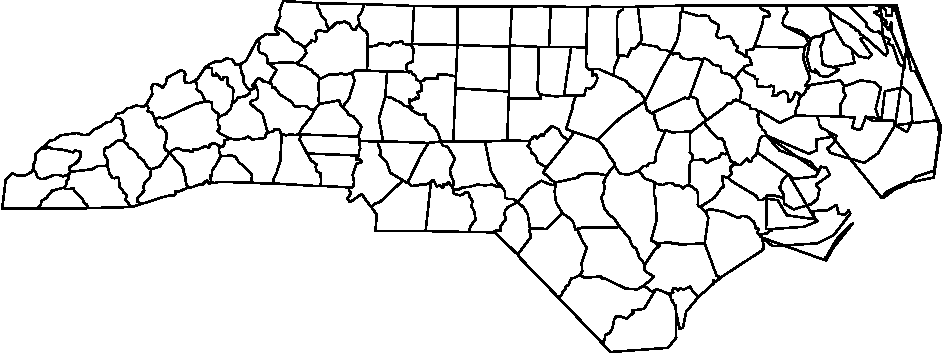
\includegraphics[width=0.95\textwidth]{Lec17_files/figure-beamer/unnamed-chunk-19-1} \end{center}

\end{frame}

\begin{frame}[fragile,t]{Grouping Features}

\scriptoutput

\begin{Shaded}
\begin{Highlighting}[]
\NormalTok{nc_state =}\StringTok{ }\KeywordTok{st_union}\NormalTok{(nc)}
\KeywordTok{plot}\NormalTok{(nc_state)}
\end{Highlighting}
\end{Shaded}

\begin{center}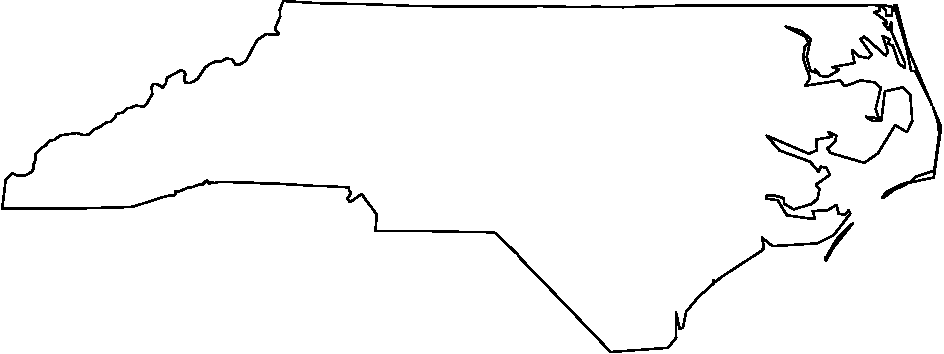
\includegraphics[width=0.95\textwidth]{Lec17_files/figure-beamer/unnamed-chunk-20-1} \end{center}

\begin{Shaded}
\begin{Highlighting}[]

\NormalTok{nc_state}
\NormalTok{## Geometry set for 1 feature }
\NormalTok{## geometry type:  MULTIPOLYGON}
\NormalTok{## dimension:      XY}
\NormalTok{## bbox:           xmin: -84.32385 ymin: 33.88199 xmax: -75.45698 ymax: 36.58965}
\NormalTok{## epsg (SRID):    4267}
\NormalTok{## proj4string:    +proj=longlat +datum=NAD27 +no_defs}
\end{Highlighting}
\end{Shaded}

\end{frame}

\begin{frame}[fragile,t]{More Grouping}

\scriptoutput

\begin{Shaded}
\begin{Highlighting}[]
\NormalTok{nc_cut =}\StringTok{ }\NormalTok{nc }\OperatorTok
\StringTok{  }\KeywordTok{cbind}\NormalTok{(nc }\OperatorTok\StringTok{ }\KeywordTok{st_centroid}\NormalTok{() }\OperatorTok\StringTok{ }\KeywordTok{st_coordinates}\NormalTok{()) }\OperatorTok
\StringTok{  }\KeywordTok{mutate}\NormalTok{(}\DataTypeTok{region =} \KeywordTok{cut}\NormalTok{(X, }\DataTypeTok{breaks =} \DecValTok{5}\NormalTok{))}

\NormalTok{nc_cut}
\NormalTok{## Simple feature collection with 100 features and 10 fields}
\NormalTok{## geometry type:  MULTIPOLYGON}
\NormalTok{## dimension:      XY}
\NormalTok{## bbox:           xmin: -84.32385 ymin: 33.88199 xmax: -75.45698 ymax: 36.58965}
\NormalTok{## epsg (SRID):    4267}
\NormalTok{## proj4string:    +proj=longlat +datum=NAD27 +no_defs}
\NormalTok{## First 20 features:}
\NormalTok{##           NAME BIR74 SID74 NWBIR74 BIR79 SID79 NWBIR79         X}
\NormalTok{## 1         Ashe  1091     1      10  1364     0      19 -81.49826}
\NormalTok{## 2    Alleghany   487     0      10   542     3      12 -81.12515}
\NormalTok{## 3        Surry  3188     5     208  3616     6     260 -80.68575}
\NormalTok{## 4    Currituck   508     1     123   830     2     145 -76.02750}
\NormalTok{## 5  Northampton  1421     9    1066  1606     3    1197 -77.41056}
\NormalTok{## 6     Hertford  1452     7     954  1838     5    1237 -76.99478}
\NormalTok{## 7       Camden   286     0     115   350     2     139 -76.23435}
\NormalTok{## 8        Gates   420     0     254   594     2     371 -76.70448}
\NormalTok{## 9       Warren   968     4     748  1190     2     844 -78.11043}
\NormalTok{## 10      Stokes  1612     1     160  2038     5     176 -80.23428}
\NormalTok{## 11     Caswell  1035     2     550  1253     2     597 -79.33477}
\NormalTok{## 12  Rockingham  4449    16    1243  5386     5    1369 -79.77038}
\NormalTok{## 13   Granville  1671     4     930  2074     4    1058 -78.65647}
\NormalTok{## 14      Person  1556     4     613  1790     4     650 -78.97684}
\NormalTok{## 15       Vance  2180     4    1179  2753     6    1492 -78.41127}
\NormalTok{## 16     Halifax  3608    18    2365  4463    17    2980 -77.65628}
\NormalTok{## 17  Pasquotank  1638     3     622  2275     4     933 -76.31460}
\NormalTok{## 18      Wilkes  3146     4     200  3725     7     222 -81.15963}
\NormalTok{## 19     Watauga  1323     1      17  1775     1      33 -81.69129}
\NormalTok{## 20  Perquimans   484     1     230   676     0     310 -76.45461}
\NormalTok{##           Y        region                       geometry}
\NormalTok{## 1  36.43140 (-82.4,-80.8] MULTIPOLYGON(((-81.47275543...}
\NormalTok{## 2  36.49101 (-82.4,-80.8] MULTIPOLYGON(((-81.23989105...}
\NormalTok{## 3  36.41252 (-80.8,-79.1] MULTIPOLYGON(((-80.45634460...}
\NormalTok{## 4  36.40728 (-77.5,-75.8] MULTIPOLYGON(((-76.00897216...}
\NormalTok{## 5  36.42228 (-77.5,-75.8] MULTIPOLYGON(((-77.21766662...}
\NormalTok{## 6  36.36145 (-77.5,-75.8] MULTIPOLYGON(((-76.74506378...}
\NormalTok{## 7  36.40120 (-77.5,-75.8] MULTIPOLYGON(((-76.00897216...}
\NormalTok{## 8  36.44423 (-77.5,-75.8] MULTIPOLYGON(((-76.56250762...}
\NormalTok{## 9  36.39697 (-79.1,-77.5] MULTIPOLYGON(((-78.30876159...}
\NormalTok{## 10 36.40034 (-80.8,-79.1] MULTIPOLYGON(((-80.02567291...}
\NormalTok{## 11 36.39347 (-80.8,-79.1] MULTIPOLYGON(((-79.53050994...}
\NormalTok{## 12 36.39600 (-80.8,-79.1] MULTIPOLYGON(((-79.53050994...}
\NormalTok{## 13 36.30013 (-79.1,-77.5] MULTIPOLYGON(((-78.74912261...}
\NormalTok{## 14 36.38870 (-79.1,-77.5] MULTIPOLYGON(((-78.80680084...}
\NormalTok{## 15 36.36234 (-79.1,-77.5] MULTIPOLYGON(((-78.49252319...}
\NormalTok{## 16 36.25305 (-79.1,-77.5] MULTIPOLYGON(((-77.33220672...}
\NormalTok{## 17 36.31237 (-77.5,-75.8] MULTIPOLYGON(((-76.29892730...}
\NormalTok{## 18 36.20160 (-82.4,-80.8] MULTIPOLYGON(((-81.02056884...}
\NormalTok{## 19 36.22480 (-82.4,-80.8] MULTIPOLYGON(((-81.80622100...}
\NormalTok{## 20 36.20488 (-77.5,-75.8] MULTIPOLYGON(((-76.48052978...}
\end{Highlighting}
\end{Shaded}

\end{frame}

\begin{frame}[fragile,t]{}

\scriptoutput

\begin{Shaded}
\begin{Highlighting}[]
\KeywordTok{ggplot}\NormalTok{(nc_cut) }\OperatorTok{+}
\StringTok{  }\KeywordTok{geom_sf}\NormalTok{(}\KeywordTok{aes}\NormalTok{(}\DataTypeTok{fill=}\NormalTok{region))}
\end{Highlighting}
\end{Shaded}

\begin{center}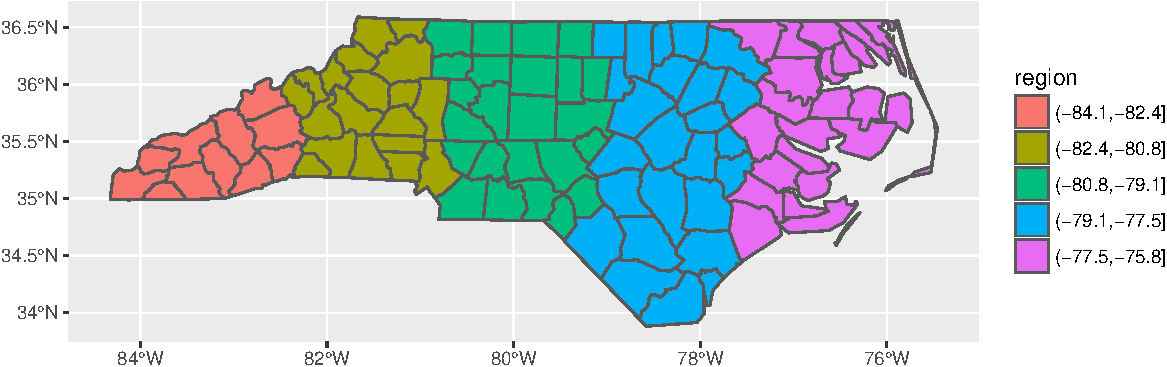
\includegraphics[width=0.95\textwidth]{Lec17_files/figure-beamer/unnamed-chunk-22-1} \end{center}

\end{frame}

\begin{frame}[fragile,t]{dplyr and sf - BFFs}

\scriptoutput

\begin{Shaded}
\begin{Highlighting}[]
\NormalTok{nc_cut }\OperatorTok\StringTok{ }
\StringTok{  }\KeywordTok{group_by}\NormalTok{(region) }\OperatorTok\StringTok{ }
\StringTok{  }\KeywordTok{summarize}\NormalTok{(}\DataTypeTok{geometry =} \KeywordTok{st_union}\NormalTok{(geometry)) }\OperatorTok\StringTok{ }
\StringTok{  }\KeywordTok{ggplot}\NormalTok{() }\OperatorTok{+}\StringTok{ }\KeywordTok{geom_sf}\NormalTok{(}\KeywordTok{aes}\NormalTok{(}\DataTypeTok{fill=}\NormalTok{region))}
\end{Highlighting}
\end{Shaded}

\begin{center}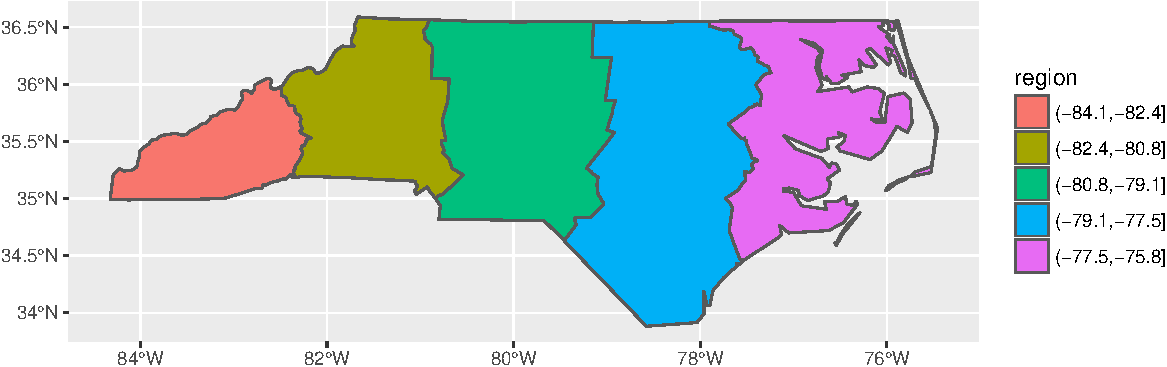
\includegraphics[width=0.95\textwidth]{Lec17_files/figure-beamer/unnamed-chunk-23-1} \end{center}

\end{frame}

\begin{frame}[fragile,t]{Affine Transfomations}

\scriptoutput

\begin{Shaded}
\begin{Highlighting}[]
\NormalTok{rotate =}\StringTok{ }\ControlFlowTok{function}\NormalTok{(a) }\KeywordTok{matrix}\NormalTok{(}\KeywordTok{c}\NormalTok{(}\KeywordTok{cos}\NormalTok{(a), }\KeywordTok{sin}\NormalTok{(a), }\OperatorTok{-}\KeywordTok{sin}\NormalTok{(a), }\KeywordTok{cos}\NormalTok{(a)), }\DecValTok{2}\NormalTok{, }\DecValTok{2}\NormalTok{)}

\NormalTok{ctrd =}\StringTok{ }\KeywordTok{st_centroid}\NormalTok{(nc_state)}
\NormalTok{state_rotate =}\StringTok{ }\NormalTok{(nc_state }\OperatorTok{-}\StringTok{ }\NormalTok{ctrd) }\OperatorTok{*}\StringTok{ }\KeywordTok{rotate}\NormalTok{(}\OperatorTok{-}\NormalTok{pi}\OperatorTok{/}\DecValTok{4}\NormalTok{) }\OperatorTok{+}\StringTok{ }\NormalTok{ctrd}
\KeywordTok{plot}\NormalTok{(state_rotate, }\DataTypeTok{axes=}\OtherTok{TRUE}\NormalTok{)}
\end{Highlighting}
\end{Shaded}

\begin{center}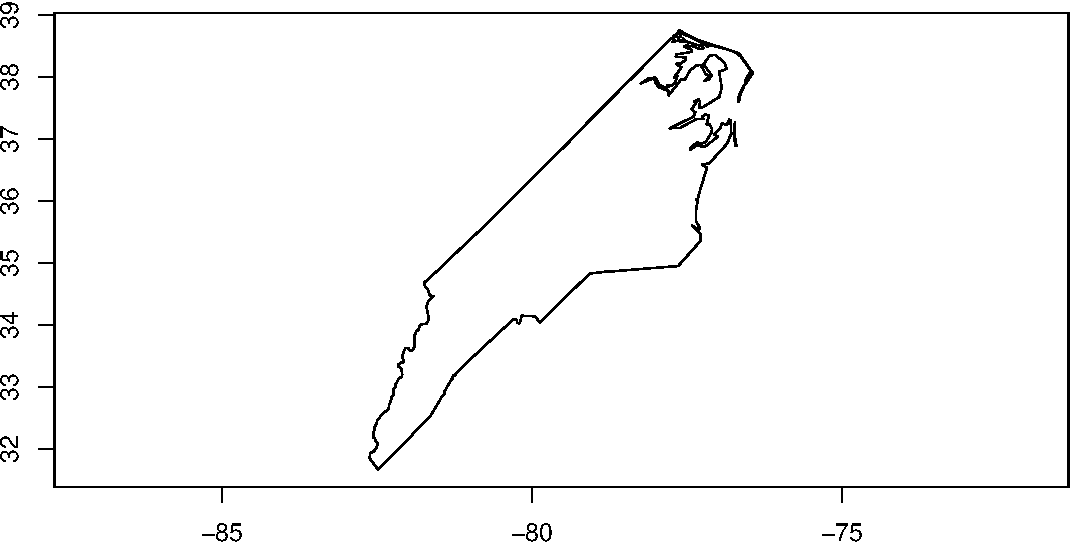
\includegraphics[width=0.95\textwidth]{Lec17_files/figure-beamer/unnamed-chunk-24-1} \end{center}

\end{frame}

\begin{frame}[fragile]{Scaling Size}

\scriptoutput

\begin{Shaded}
\begin{Highlighting}[]
\NormalTok{ctrd =}\StringTok{ }\KeywordTok{st_geometry}\NormalTok{(}\KeywordTok{st_centroid}\NormalTok{(nc))}
\NormalTok{area =}\StringTok{ }\KeywordTok{st_area}\NormalTok{(nc) }\OperatorTok\StringTok{ }\KeywordTok{strip_attrs}\NormalTok{()}
\NormalTok{nc_scaled =}\StringTok{ }\NormalTok{nc}
\ControlFlowTok{for}\NormalTok{(i }\ControlFlowTok{in} \DecValTok{1}\OperatorTok{:}\KeywordTok{nrow}\NormalTok{(nc))}
\NormalTok{  nc_scaled}\OperatorTok{$}\NormalTok{geometry[[i]] =}\StringTok{ }\NormalTok{((}\KeywordTok{st_geometry}\NormalTok{(nc[i,]) }\OperatorTok{-}\StringTok{ }\NormalTok{ctrd[i]) }\OperatorTok{*}
\StringTok{                               }\KeywordTok{sqrt}\NormalTok{(}\KeywordTok{min}\NormalTok{(area)}\OperatorTok{/}\NormalTok{area[i]) }\OperatorTok{+}\StringTok{ }\NormalTok{ctrd[i])[[}\DecValTok{1}\NormalTok{]]}

\KeywordTok{plot}\NormalTok{(nc_scaled[,}\StringTok{"SID79"}\NormalTok{])}
\end{Highlighting}
\end{Shaded}

\begin{center}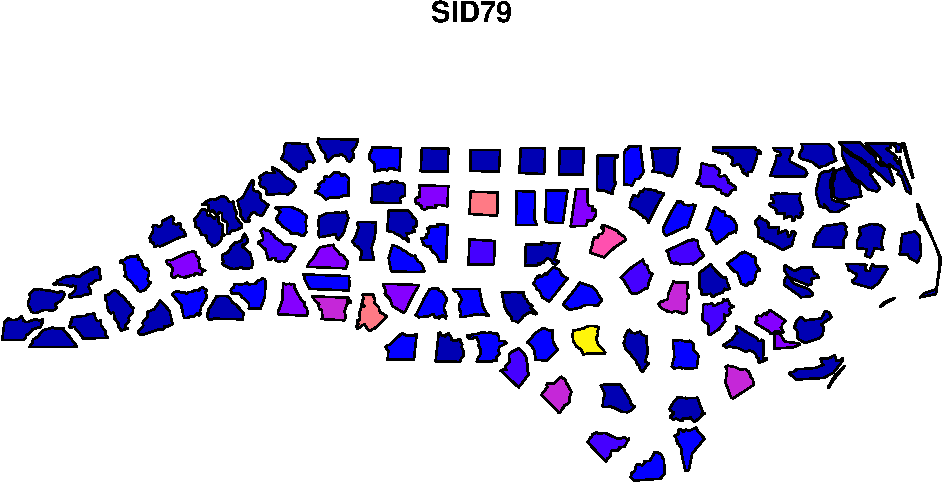
\includegraphics[width=0.95\textwidth]{Lec17_files/figure-beamer/unnamed-chunk-25-1} \end{center}

\end{frame}

\begin{frame}[fragile,t]{Back to the highways}

\scriptoutput

\begin{Shaded}
\begin{Highlighting}[]
\NormalTok{hwy =}\StringTok{ }\KeywordTok{st_read}\NormalTok{(}\StringTok{"../../data/gis/us_interstates/"}\NormalTok{, }\DataTypeTok{quiet=}\OtherTok{TRUE}\NormalTok{, }\DataTypeTok{stringsAsFactors=}\OtherTok{FALSE}\NormalTok{) }\OperatorTok\StringTok{ }\KeywordTok{st_transform}\NormalTok{(}\KeywordTok{st_crs}\NormalTok{(nc))}

\KeywordTok{ggplot}\NormalTok{() }\OperatorTok{+}
\StringTok{  }\KeywordTok{geom_sf}\NormalTok{(}\DataTypeTok{data=}\NormalTok{nc) }\OperatorTok{+}
\StringTok{  }\KeywordTok{geom_sf}\NormalTok{(}\DataTypeTok{data=}\NormalTok{hwy, }\DataTypeTok{col=}\StringTok{'red'}\NormalTok{)}
\end{Highlighting}
\end{Shaded}

\begin{center}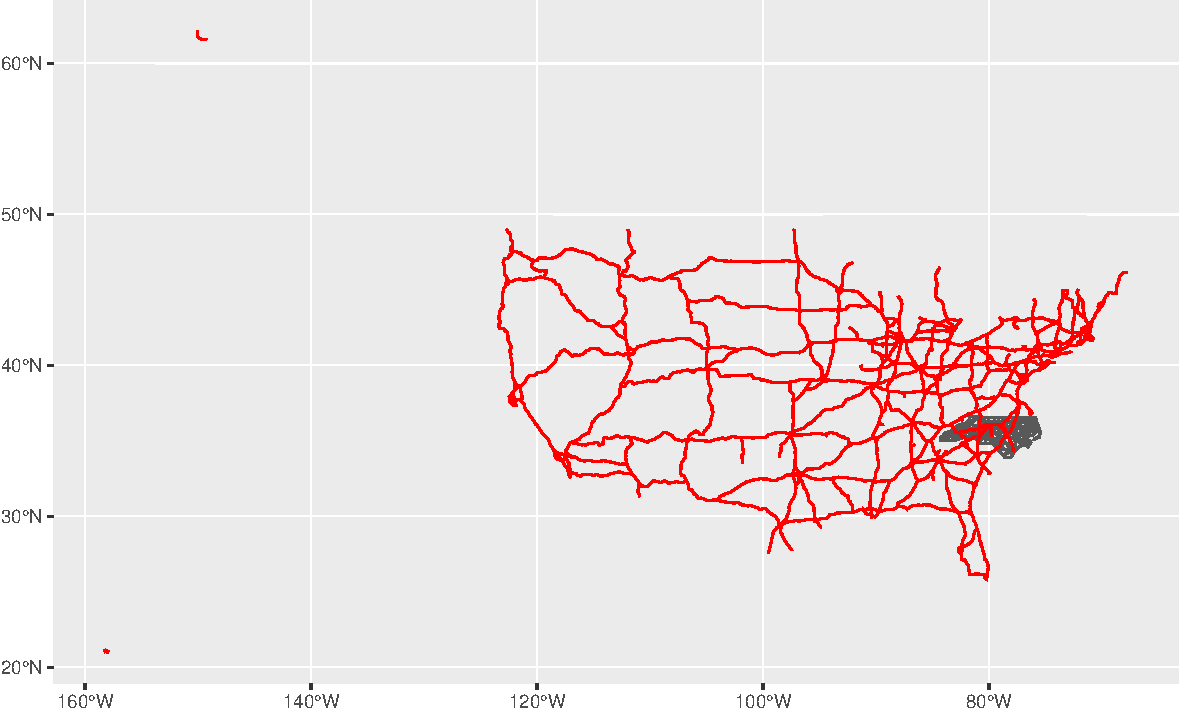
\includegraphics[width=0.95\textwidth]{Lec17_files/figure-beamer/unnamed-chunk-26-1} \end{center}

\end{frame}

\begin{frame}[fragile,t]{NC Interstate Highways}

\scriptoutput

\begin{Shaded}
\begin{Highlighting}[]
\NormalTok{hwy_nc =}\StringTok{ }\KeywordTok{st_intersection}\NormalTok{(hwy, nc)}

\KeywordTok{ggplot}\NormalTok{() }\OperatorTok{+}\StringTok{ }
\StringTok{  }\KeywordTok{geom_sf}\NormalTok{(}\DataTypeTok{data=}\NormalTok{nc) }\OperatorTok{+}
\StringTok{  }\KeywordTok{geom_sf}\NormalTok{(}\DataTypeTok{data=}\NormalTok{hwy_nc, }\DataTypeTok{col=}\StringTok{'red'}\NormalTok{)}
\end{Highlighting}
\end{Shaded}

\begin{center}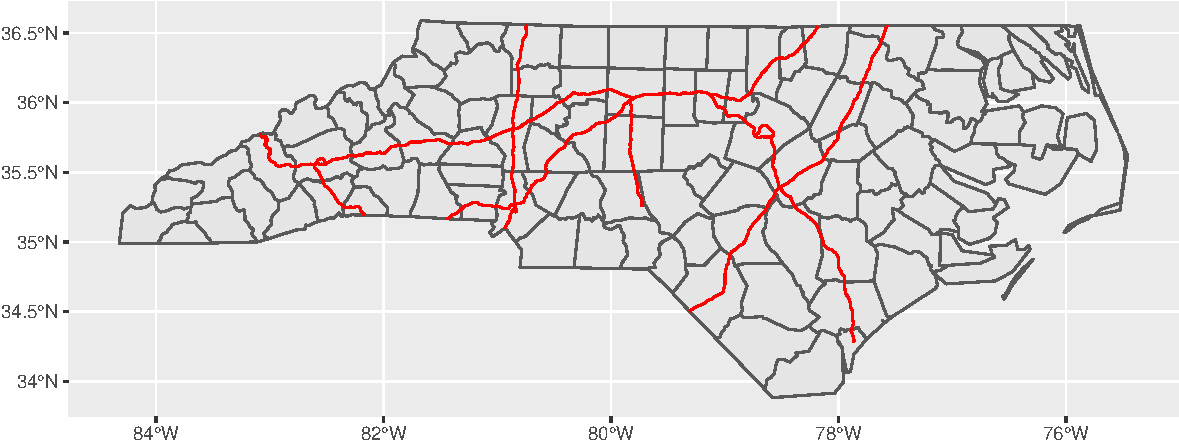
\includegraphics[width=0.95\textwidth]{Lec17_files/figure-beamer/unnamed-chunk-27-1} \end{center}

\begin{Shaded}
\begin{Highlighting}[]

\NormalTok{hwy_nc}
\NormalTok{## Simple feature collection with 56 features and 10 fields}
\NormalTok{## geometry type:  GEOMETRY}
\NormalTok{## dimension:      XY}
\NormalTok{## bbox:           xmin: -83.09008 ymin: 34.2791 xmax: -77.57348 ymax: 36.56092}
\NormalTok{## epsg (SRID):    4267}
\NormalTok{## proj4string:    +proj=longlat +datum=NAD27 +no_defs}
\NormalTok{## First 20 features:}
\NormalTok{##    ROUTE_NUM DIST_MILES DIST_KM        NAME BIR74 SID74 NWBIR74 BIR79}
\NormalTok{## 1        I77     546.83  880.05       Surry  3188     5     208  3616}
\NormalTok{## 2        I95    1829.69 2944.61 Northampton  1421     9    1066  1606}
\NormalTok{## 3        I85     610.51  982.53      Warren   968     4     748  1190}
\NormalTok{## 4        I85     610.51  982.53   Granville  1671     4     930  2074}
\NormalTok{## 5        I85     610.51  982.53       Vance  2180     4    1179  2753}
\NormalTok{## 6        I95    1829.69 2944.61     Halifax  3608    18    2365  4463}
\NormalTok{## 7        I77     546.83  880.05      Yadkin  1269     1      65  1568}
\NormalTok{## 8        I40    2480.59 3992.14     Forsyth 11858    10    3919 15704}
\NormalTok{## 9     I40  F      18.33   29.49     Forsyth 11858    10    3919 15704}
\NormalTok{## 10       I40    2480.59 3992.14    Guilford 16184    23    5483 20543}
\NormalTok{## 11    I40  F      18.33   29.49    Guilford 16184    23    5483 20543}
\NormalTok{## 12       I73      54.84   88.25    Guilford 16184    23    5483 20543}
\NormalTok{## 13       I85     610.51  982.53    Guilford 16184    23    5483 20543}
\NormalTok{## 14       I40    2480.59 3992.14    Alamance  4672    13    1243  5767}
\NormalTok{## 15       I85     610.51  982.53    Alamance  4672    13    1243  5767}
\NormalTok{## 16       I40    2480.59 3992.14      Orange  3164     4     776  4478}
\NormalTok{## 17       I85     610.51  982.53      Orange  3164     4     776  4478}
\NormalTok{## 18       I40    2480.59 3992.14      Durham  7970    16    3732 10432}
\NormalTok{## 19       I85     610.51  982.53      Durham  7970    16    3732 10432}
\NormalTok{## 20       I95    1829.69 2944.61        Nash  4021     8    1851  5189}
\NormalTok{##    SID79 NWBIR79                          geoms}
\NormalTok{## 1      6     260 LINESTRING(-80.745014063930...}
\NormalTok{## 2      3    1197 LINESTRING(-77.57347527372 ...}
\NormalTok{## 3      2     844 LINESTRING(-78.303117397331...}
\NormalTok{## 4      4    1058 LINESTRING(-78.788842681252...}
\NormalTok{## 5      6    1492 LINESTRING(-78.515924528417...}
\NormalTok{## 6     17    2980 LINESTRING(-77.629052087089...}
\NormalTok{## 7      1      76 LINESTRING(-80.819025924954...}
\NormalTok{## 8     18    5031 LINESTRING(-80.425019190468...}
\NormalTok{## 9     18    5031 LINESTRING(-80.325561526296...}
\NormalTok{## 10    38    7089 LINESTRING(-80.007026428880...}
\NormalTok{## 11    38    7089 LINESTRING(-80.033752259421...}
\NormalTok{## 12    38    7089 LINESTRING(-79.826140362816...}
\NormalTok{## 13    38    7089 LINESTRING(-79.804892355469...}
\NormalTok{## 14    11    1397 MULTILINESTRING((-79.259665...}
\NormalTok{## 15    11    1397 LINESTRING(-79.261130125158...}
\NormalTok{## 16     6    1086 LINESTRING(-79.259586126259...}
\NormalTok{## 17     6    1086 LINESTRING(-79.125632056119...}
\NormalTok{## 18    22    4948 LINESTRING(-79.001499734474...}
\NormalTok{## 19    22    4948 LINESTRING(-78.986039485815...}
\NormalTok{## 20     7    2274 LINESTRING(-77.786676909027...}
\end{Highlighting}
\end{Shaded}

\end{frame}

\begin{frame}[fragile,t]{Counties near the interstate (Projection)}

\scriptoutput

\begin{Shaded}
\begin{Highlighting}[]
\NormalTok{nc_utm  =}\StringTok{ }\KeywordTok{st_transform}\NormalTok{(nc,  }\StringTok{"+proj=utm +zone=17 +datum=NAD83 +units=m +no_defs"}\NormalTok{)}
\NormalTok{hwy_utm =}\StringTok{ }\KeywordTok{st_transform}\NormalTok{(hwy, }\StringTok{"+proj=utm +zone=17 +datum=NAD83 +units=m +no_defs"}\NormalTok{)}

\NormalTok{hwy_nc_utm =}\StringTok{ }\KeywordTok{st_intersection}\NormalTok{(nc_utm, hwy_utm)}

\KeywordTok{ggplot}\NormalTok{() }\OperatorTok{+}\StringTok{ }
\StringTok{  }\KeywordTok{geom_sf}\NormalTok{(}\DataTypeTok{data=}\NormalTok{nc_utm) }\OperatorTok{+}
\StringTok{  }\KeywordTok{geom_sf}\NormalTok{(}\DataTypeTok{data=}\NormalTok{hwy_nc_utm, }\DataTypeTok{col=}\StringTok{'red'}\NormalTok{)}
\end{Highlighting}
\end{Shaded}

\begin{center}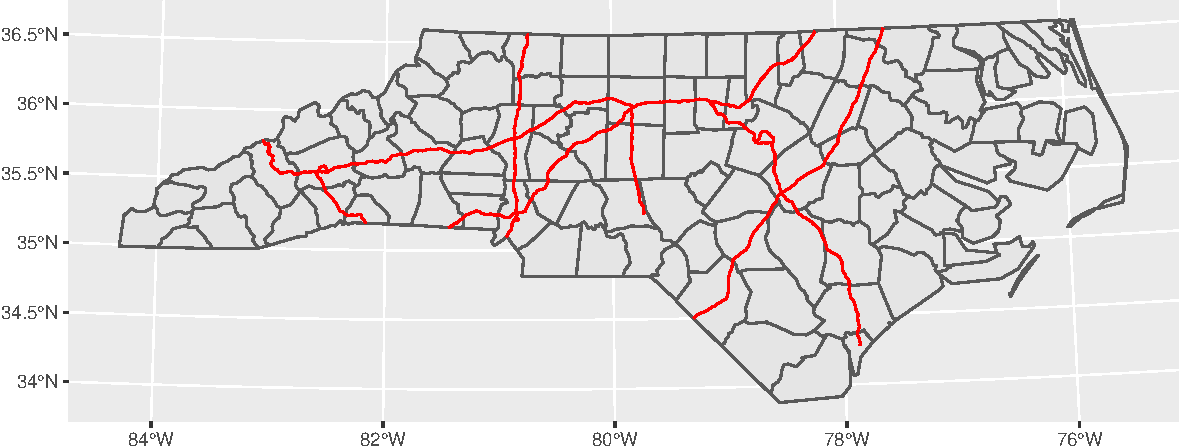
\includegraphics[width=0.95\textwidth]{Lec17_files/figure-beamer/unnamed-chunk-28-1} \end{center}

\end{frame}

\begin{frame}[fragile,t]{Counties near the interstate (Buffering)}

\scriptoutput

\begin{Shaded}
\begin{Highlighting}[]
\NormalTok{hwy_nc_buffer =}\StringTok{ }\KeywordTok{st_buffer}\NormalTok{(hwy_nc_utm, }\DecValTok{10000}\NormalTok{)}

\KeywordTok{ggplot}\NormalTok{() }\OperatorTok{+}\StringTok{ }
\StringTok{  }\KeywordTok{geom_sf}\NormalTok{(}\DataTypeTok{data=}\NormalTok{nc_utm) }\OperatorTok{+}
\StringTok{  }\KeywordTok{geom_sf}\NormalTok{(}\DataTypeTok{data=}\NormalTok{hwy_nc_utm, }\DataTypeTok{color=}\StringTok{'red'}\NormalTok{) }\OperatorTok{+}
\StringTok{  }\KeywordTok{geom_sf}\NormalTok{(}\DataTypeTok{data=}\NormalTok{hwy_nc_buffer, }\DataTypeTok{fill=}\StringTok{'red'}\NormalTok{, }\DataTypeTok{alpha=}\FloatTok{0.3}\NormalTok{)}
\end{Highlighting}
\end{Shaded}

\begin{center}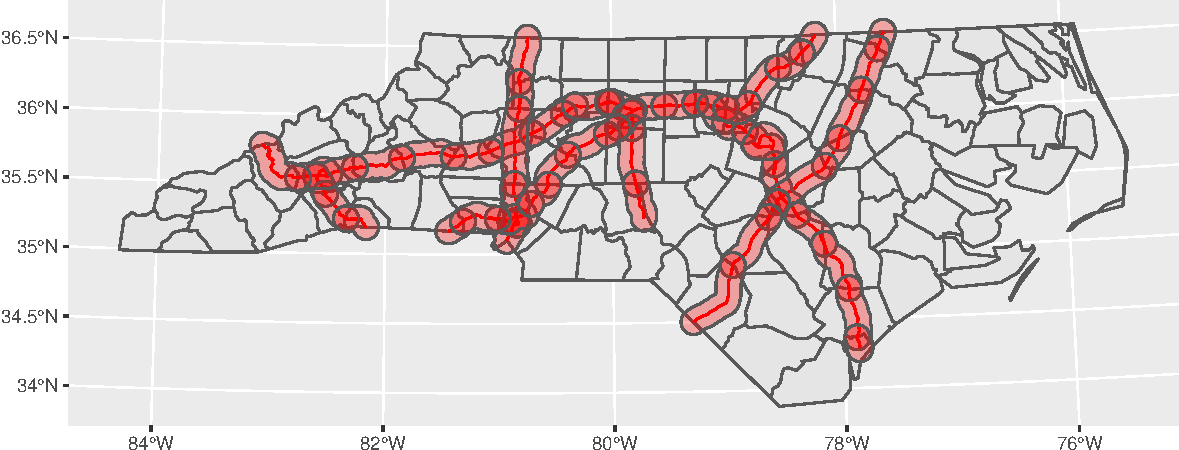
\includegraphics[width=0.95\textwidth]{Lec17_files/figure-beamer/unnamed-chunk-29-1} \end{center}

\end{frame}

\begin{frame}[fragile,t]{Counties near the interstate (Buffering +
Union)}

\scriptoutput

\begin{Shaded}
\begin{Highlighting}[]
\NormalTok{hwy_nc_buffer =}\StringTok{ }\KeywordTok{st_buffer}\NormalTok{(hwy_nc_utm, }\DecValTok{10000}\NormalTok{) }\OperatorTok\StringTok{ }\KeywordTok{st_union}\NormalTok{() }\OperatorTok\StringTok{ }\KeywordTok{st_sf}\NormalTok{()}

\KeywordTok{ggplot}\NormalTok{() }\OperatorTok{+}\StringTok{ }
\StringTok{  }\KeywordTok{geom_sf}\NormalTok{(}\DataTypeTok{data=}\NormalTok{nc_utm) }\OperatorTok{+}
\StringTok{  }\KeywordTok{geom_sf}\NormalTok{(}\DataTypeTok{data=}\NormalTok{hwy_nc_utm, }\DataTypeTok{color=}\StringTok{'red'}\NormalTok{) }\OperatorTok{+}
\StringTok{  }\KeywordTok{geom_sf}\NormalTok{(}\DataTypeTok{data=}\NormalTok{hwy_nc_buffer, }\DataTypeTok{fill=}\StringTok{'red'}\NormalTok{, }\DataTypeTok{alpha=}\FloatTok{0.3}\NormalTok{)}
\end{Highlighting}
\end{Shaded}

\begin{center}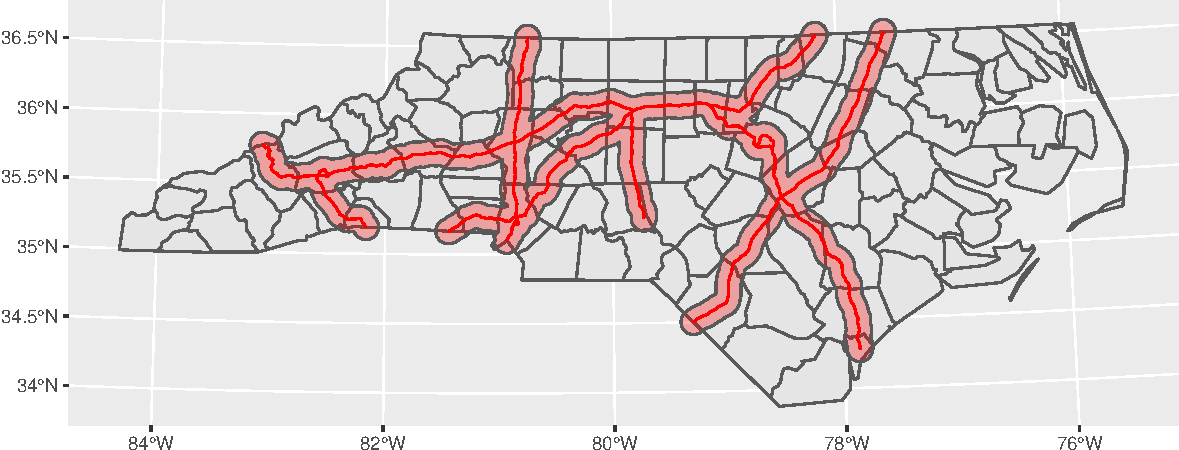
\includegraphics[width=0.95\textwidth]{Lec17_files/figure-beamer/unnamed-chunk-30-1} \end{center}

\end{frame}

\begin{frame}[t]{Exercise 1}

How many counties in North Carolina are within 5, 10, 20, or 50 km of an
interstate highway?

\end{frame}

\section{Raster Data}\label{raster-data}

\begin{frame}[fragile,t]{Example data - Meuse}

\scriptoutput

\begin{Shaded}
\begin{Highlighting}[]
\NormalTok{meuse_rast =}\StringTok{ }\KeywordTok{raster}\NormalTok{(}\KeywordTok{system.file}\NormalTok{(}\StringTok{"external/test.grd"}\NormalTok{, }\DataTypeTok{package=}\StringTok{"raster"}\NormalTok{))}

\NormalTok{meuse_rast}
\NormalTok{## class       : RasterLayer }
\NormalTok{## dimensions  : 115, 80, 9200  (nrow, ncol, ncell)}
\NormalTok{## resolution  : 40, 40  (x, y)}
\NormalTok{## extent      : 178400, 181600, 329400, 334000  (xmin, xmax, ymin, ymax)}
\NormalTok{## coord. ref. : +init=epsg:28992 +towgs84=565.237,50.0087,465.658,-0.406857,0.350733,-1.87035,4.0812 +proj=sterea +lat_0=52.15616055555555 +lon_0=5.38763888888889 +k=0.9999079 +x_0=155000 +y_0=463000 +ellps=bessel +units=m +no_defs }
\NormalTok{## data source : /usr/local/lib/R/3.3/site-library/raster/external/test.grd }
\NormalTok{## names       : test }
\NormalTok{## values      : 128.434, 1805.78  (min, max)}
\end{Highlighting}
\end{Shaded}

\end{frame}

\begin{frame}[fragile,t]{}

\scriptoutput

\begin{Shaded}
\begin{Highlighting}[]
\KeywordTok{plot}\NormalTok{(meuse_rast)}
\KeywordTok{plot}\NormalTok{(meuse_riv, }\DataTypeTok{add=}\OtherTok{TRUE}\NormalTok{, }\DataTypeTok{col=}\KeywordTok{adjustcolor}\NormalTok{(}\StringTok{"lightblue"}\NormalTok{,}\DataTypeTok{alpha.f =} \FloatTok{0.5}\NormalTok{), }\DataTypeTok{border=}\OtherTok{NA}\NormalTok{)}
\end{Highlighting}
\end{Shaded}

\begin{center}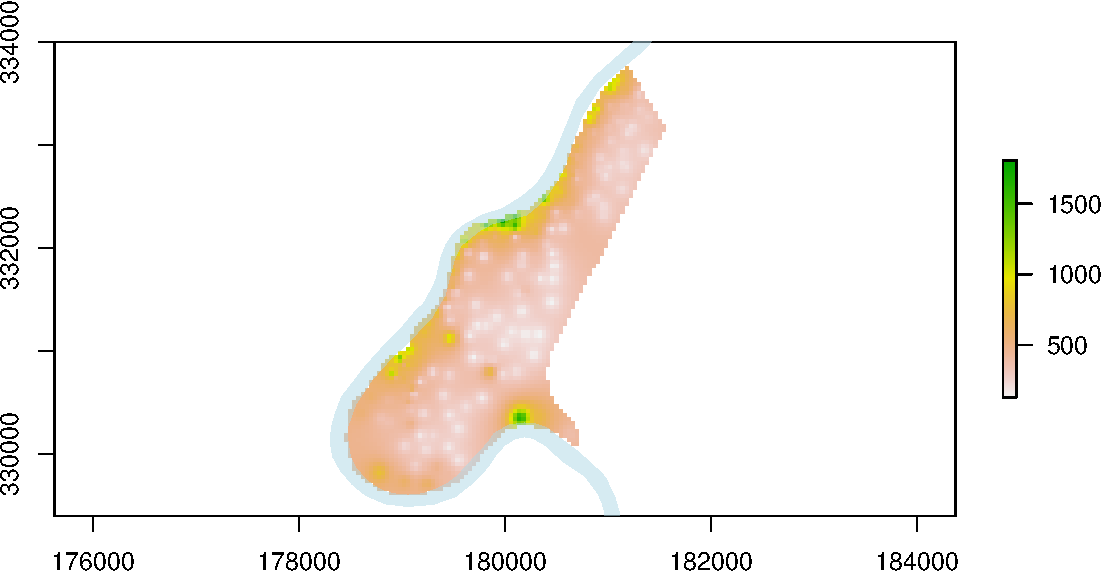
\includegraphics[width=0.95\textwidth]{Lec17_files/figure-beamer/unnamed-chunk-32-1} \end{center}

\end{frame}

\begin{frame}[fragile]{raster class}

\begin{Shaded}
\begin{Highlighting}[]
\KeywordTok{str}\NormalTok{(meuse_rast)}
\NormalTok{## Formal class 'RasterLayer' [package "raster"] with 12 slots}
\NormalTok{##   ..@ file    :Formal class '.RasterFile' [package "raster"] with 13 slots}
\NormalTok{##   .. .. ..@ name        : chr "/usr/local/lib/R/3.3/site-library/raster/external/test.grd"}
\NormalTok{##   .. .. ..@ datanotation: chr "FLT4S"}
\NormalTok{##   .. .. ..@ byteorder   : Named chr "little"}
\NormalTok{##   .. .. .. ..- attr(*, "names")= chr "value"}
\NormalTok{##   .. .. ..@ nodatavalue : num -3.4e+38}
\NormalTok{##   .. .. ..@ NAchanged   : logi FALSE}
\NormalTok{##   .. .. ..@ nbands      : int 1}
\NormalTok{##   .. .. ..@ bandorder   : Named chr "BIL"}
\NormalTok{##   .. .. .. ..- attr(*, "names")= chr "value"}
\NormalTok{##   .. .. ..@ offset      : int 0}
\NormalTok{##   .. .. ..@ toptobottom : logi TRUE}
\NormalTok{##   .. .. ..@ blockrows   : int 0}
\NormalTok{##   .. .. ..@ blockcols   : int 0}
\NormalTok{##   .. .. ..@ driver      : chr "raster"}
\NormalTok{##   .. .. ..@ open        : logi FALSE}
\NormalTok{##   ..@ data    :Formal class '.SingleLayerData' [package "raster"] with 13 slots}
\NormalTok{##   .. .. ..@ values    : logi(0) }
\NormalTok{##   .. .. ..@ offset    : num 0}
\NormalTok{##   .. .. ..@ gain      : num 1}
\NormalTok{##   .. .. ..@ inmemory  : logi FALSE}
\NormalTok{##   .. .. ..@ fromdisk  : logi TRUE}
\NormalTok{##   .. .. ..@ isfactor  : logi FALSE}
\NormalTok{##   .. .. ..@ attributes: list()}
\NormalTok{##   .. .. ..@ haveminmax: logi TRUE}
\NormalTok{##   .. .. ..@ min       : num 128}
\NormalTok{##   .. .. ..@ max       : num 1806}
\NormalTok{##   .. .. ..@ band      : int 1}
\NormalTok{##   .. .. ..@ unit      : chr ""}
\NormalTok{##   .. .. ..@ names     : chr "test"}
\NormalTok{##   ..@ legend  :Formal class '.RasterLegend' [package "raster"] with 5 slots}
\NormalTok{##   .. .. ..@ type      : chr(0) }
\NormalTok{##   .. .. ..@ values    : logi(0) }
\NormalTok{##   .. .. ..@ color     : logi(0) }
\NormalTok{##   .. .. ..@ names     : logi(0) }
\NormalTok{##   .. .. ..@ colortable: logi(0) }
\NormalTok{##   ..@ title   : chr(0) }
\NormalTok{##   ..@ extent  :Formal class 'Extent' [package "raster"] with 4 slots}
\NormalTok{##   .. .. ..@ xmin: num 178400}
\NormalTok{##   .. .. ..@ xmax: num 181600}
\NormalTok{##   .. .. ..@ ymin: num 329400}
\NormalTok{##   .. .. ..@ ymax: num 334000}
\NormalTok{##   ..@ rotated : logi FALSE}
\NormalTok{##   ..@ rotation:Formal class '.Rotation' [package "raster"] with 2 slots}
\NormalTok{##   .. .. ..@ geotrans: num(0) }
\NormalTok{##   .. .. ..@ transfun:function ()  }
\NormalTok{##   ..@ ncols   : int 80}
\NormalTok{##   ..@ nrows   : int 115}
\NormalTok{##   ..@ crs     :Formal class 'CRS' [package "sp"] with 1 slot}
\NormalTok{##   .. .. ..@ projargs: chr "+init=epsg:28992 +towgs84=565.237,50.0087,465.658,-0.406857,0.350733,-1.87035,4.0812 +proj=sterea +lat_0=52.15616055555555 +lon"| __truncated__}
\NormalTok{##   ..@ history : list()}
\NormalTok{##   ..@ z       : list()}
\end{Highlighting}
\end{Shaded}

\end{frame}

\begin{frame}[fragile,t]{raster features}

\scriptoutput

\begin{Shaded}
\begin{Highlighting}[]
\KeywordTok{extent}\NormalTok{(meuse_rast)}
\NormalTok{## class       : Extent }
\NormalTok{## xmin        : 178400 }
\NormalTok{## xmax        : 181600 }
\NormalTok{## ymin        : 329400 }
\NormalTok{## ymax        : 334000}

\KeywordTok{dim}\NormalTok{(meuse_rast)}
\NormalTok{## [1] 115  80   1}

\KeywordTok{res}\NormalTok{(meuse_rast)}
\NormalTok{## [1] 40 40}

\KeywordTok{projection}\NormalTok{(meuse_rast)}
\NormalTok{## [1] "+init=epsg:28992 +towgs84=565.237,50.0087,465.658,-0.406857,0.350733,-1.87035,4.0812 +proj=sterea +lat_0=52.15616055555555 +lon_0=5.38763888888889 +k=0.9999079 +x_0=155000 +y_0=463000 +ellps=bessel +units=m +no_defs"}

\NormalTok{meuse_rast[}\DecValTok{20}\NormalTok{,]}
\NormalTok{##  [1]      NA      NA      NA      NA      NA      NA      NA      NA}
\NormalTok{##  [9]      NA      NA      NA      NA      NA      NA      NA      NA}
\NormalTok{## [17]      NA      NA      NA      NA      NA      NA      NA      NA}
\NormalTok{## [25]      NA      NA      NA      NA      NA      NA      NA      NA}
\NormalTok{## [33]      NA      NA      NA      NA      NA      NA      NA      NA}
\NormalTok{## [41]      NA      NA      NA      NA      NA      NA      NA      NA}
\NormalTok{## [49]      NA      NA      NA      NA      NA      NA      NA      NA}
\NormalTok{## [57]      NA      NA      NA 749.536 895.292 791.145 607.186 511.044}
\NormalTok{## [65] 468.404 399.325 350.362 306.180 300.483 310.082 283.940 285.771}
\NormalTok{## [73] 304.709 309.690 301.799 308.753 328.357 345.611      NA      NA}
\end{Highlighting}
\end{Shaded}

\end{frame}

\begin{frame}[fragile,t]{Rasters and Projections}

\scriptoutput

\begin{Shaded}
\begin{Highlighting}[]
\NormalTok{meuse_rast_ll =}\StringTok{ }\KeywordTok{projectRaster}\NormalTok{(meuse_rast, }\DataTypeTok{crs=}\StringTok{"+proj=longlat +datum=NAD27 +no_defs"}\NormalTok{)}

\KeywordTok{par}\NormalTok{(}\DataTypeTok{mfrow=}\KeywordTok{c}\NormalTok{(}\DecValTok{1}\NormalTok{,}\DecValTok{2}\NormalTok{))}
\KeywordTok{plot}\NormalTok{(meuse_rast)}
\KeywordTok{plot}\NormalTok{(meuse_rast_ll)}
\end{Highlighting}
\end{Shaded}

\begin{center}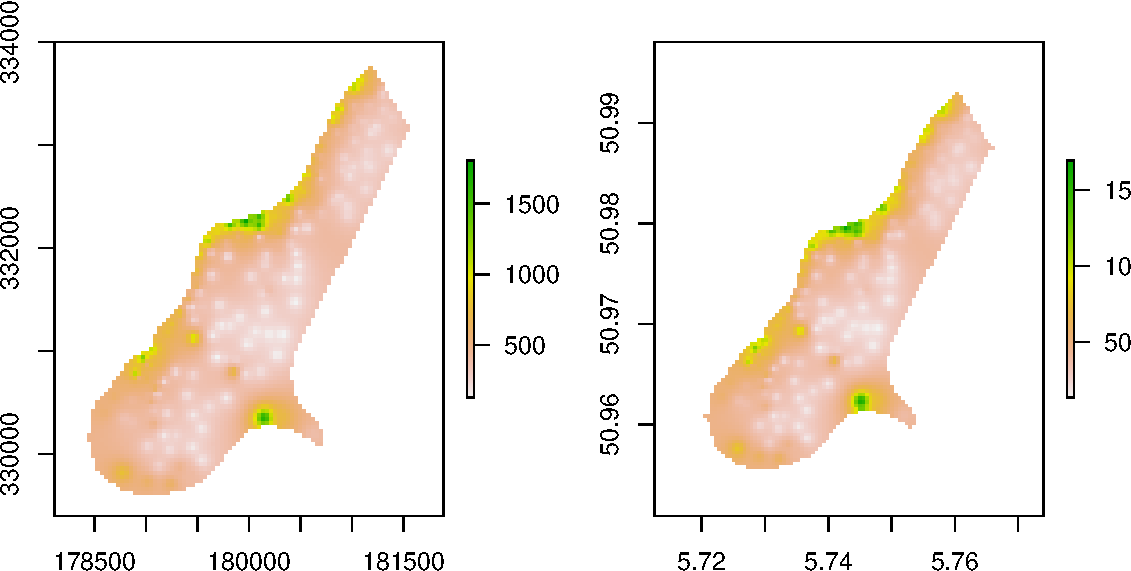
\includegraphics[width=0.95\textwidth]{Lec17_files/figure-beamer/unnamed-chunk-35-1} \end{center}

\end{frame}

\begin{frame}[fragile,t]{}

\scriptoutput

\begin{Shaded}
\begin{Highlighting}[]
\NormalTok{meuse_rast}
\NormalTok{## class       : RasterLayer }
\NormalTok{## dimensions  : 115, 80, 9200  (nrow, ncol, ncell)}
\NormalTok{## resolution  : 40, 40  (x, y)}
\NormalTok{## extent      : 178400, 181600, 329400, 334000  (xmin, xmax, ymin, ymax)}
\NormalTok{## coord. ref. : +init=epsg:28992 +towgs84=565.237,50.0087,465.658,-0.406857,0.350733,-1.87035,4.0812 +proj=sterea +lat_0=52.15616055555555 +lon_0=5.38763888888889 +k=0.9999079 +x_0=155000 +y_0=463000 +ellps=bessel +units=m +no_defs }
\NormalTok{## data source : /usr/local/lib/R/3.3/site-library/raster/external/test.grd }
\NormalTok{## names       : test }
\NormalTok{## values      : 128.434, 1805.78  (min, max)}

\NormalTok{meuse_rast_ll}
\NormalTok{## class       : RasterLayer }
\NormalTok{## dimensions  : 131, 91, 11921  (nrow, ncol, ncell)}
\NormalTok{## resolution  : 0.000569, 0.00036  (x, y)}
\NormalTok{## extent      : 5.717362, 5.769141, 50.95089, 50.99805  (xmin, xmax, ymin, ymax)}
\NormalTok{## coord. ref. : +proj=longlat +datum=NAD27 +no_defs +ellps=clrk66 +nadgrids=@conus,@alaska,@ntv2_0.gsb,@ntv1_can.dat }
\NormalTok{## data source : in memory}
\NormalTok{## names       : test }
\NormalTok{## values      : 135.647, 1693.578  (min, max)}
\end{Highlighting}
\end{Shaded}

\end{frame}

\begin{frame}[fragile,t]{Simple Features \(\longleftrightarrow\)
Rasters}

\scriptoutput

\begin{Shaded}
\begin{Highlighting}[]
\NormalTok{meuse_riv_rast =}\StringTok{ }\KeywordTok{rasterize}\NormalTok{(meuse_riv, meuse_rast)}
\NormalTok{## Error in (function (classes, fdef, mtable) : unable to find an inherited method for function 'rasterize' for signature '"sfc_POLYGON", "RasterLayer"'}

\NormalTok{meuse_riv_rast =}\StringTok{ }\KeywordTok{rasterize}\NormalTok{(}\KeywordTok{as}\NormalTok{(meuse_riv, }\StringTok{"Spatial"}\NormalTok{), meuse_rast)}
\KeywordTok{plot}\NormalTok{(meuse_riv_rast)}
\end{Highlighting}
\end{Shaded}

\begin{center}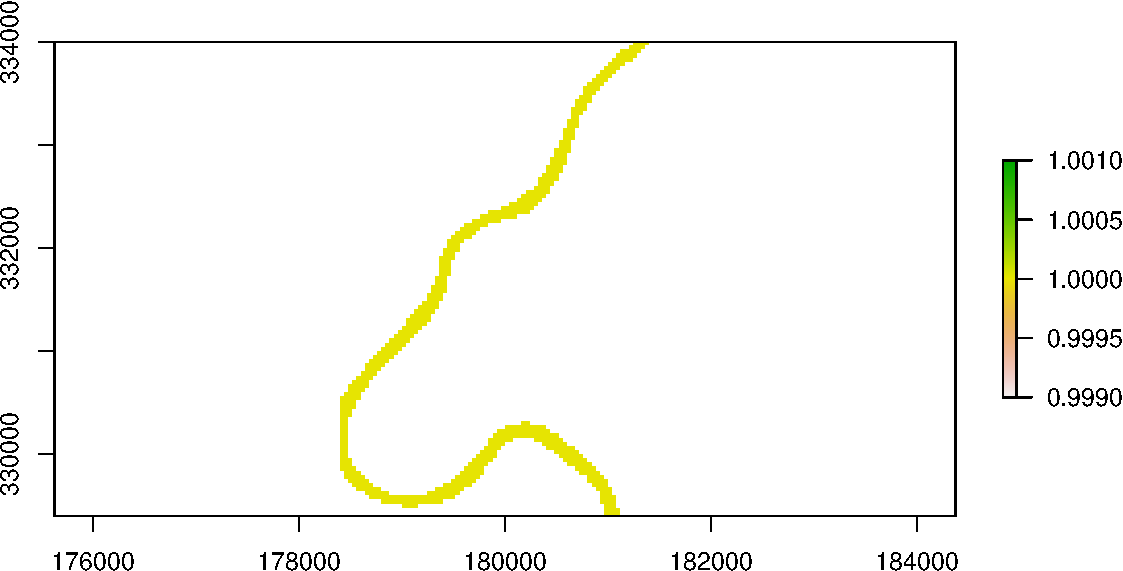
\includegraphics[width=0.95\textwidth]{Lec17_files/figure-beamer/unnamed-chunk-37-1} \end{center}

\end{frame}

\begin{frame}[fragile,t]{}

\scriptoutput

\begin{Shaded}
\begin{Highlighting}[]
\NormalTok{sub =}\StringTok{ }\OperatorTok{!}\KeywordTok{is.na}\NormalTok{(meuse_riv_rast[]) }\OperatorTok{&}\StringTok{ }\OperatorTok{!}\KeywordTok{is.na}\NormalTok{(meuse_rast[])}

\NormalTok{river_obs =}\StringTok{ }\NormalTok{meuse_rast}
\NormalTok{river_obs[}\OperatorTok{!}\NormalTok{sub] =}\StringTok{ }\OtherTok{NA}

\KeywordTok{plot}\NormalTok{(river_obs)}
\end{Highlighting}
\end{Shaded}

\begin{center}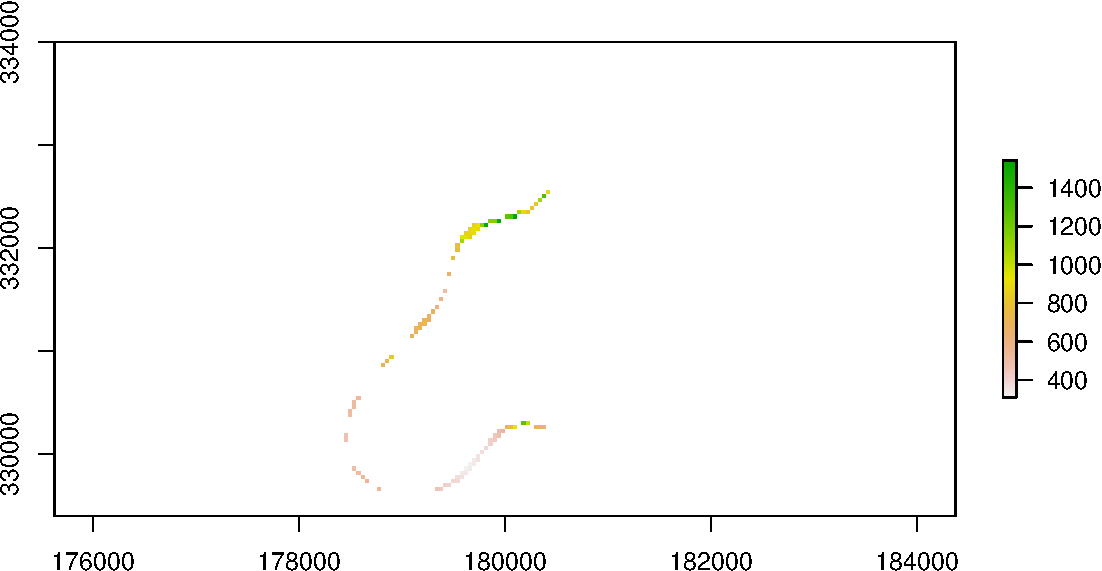
\includegraphics[width=0.95\textwidth]{Lec17_files/figure-beamer/unnamed-chunk-38-1} \end{center}

\begin{Shaded}
\begin{Highlighting}[]

\KeywordTok{xyFromCell}\NormalTok{(river_obs, }\KeywordTok{which}\NormalTok{(sub))}
\NormalTok{##            x      y}
\NormalTok{##  [1,] 180420 332540}
\NormalTok{##  [2,] 180380 332500}
\NormalTok{##  [3,] 180340 332460}
\NormalTok{##  [4,] 180300 332420}
\NormalTok{##  [5,] 180260 332380}
\NormalTok{##  [6,] 180140 332340}
\NormalTok{##  [7,] 180180 332340}
\NormalTok{##  [8,] 180220 332340}
\NormalTok{##  [9,] 180020 332300}
\NormalTok{## [10,] 180060 332300}
\NormalTok{## [11,] 180100 332300}
\NormalTok{## [12,] 179860 332260}
\NormalTok{## [13,] 179900 332260}
\NormalTok{## [14,] 179940 332260}
\NormalTok{## [15,] 179700 332220}
\NormalTok{## [16,] 179740 332220}
\NormalTok{## [17,] 179780 332220}
\NormalTok{## [18,] 179820 332220}
\NormalTok{## [19,] 179660 332180}
\NormalTok{## [20,] 179700 332180}
\NormalTok{## [21,] 179740 332180}
\NormalTok{## [22,] 179620 332140}
\NormalTok{## [23,] 179660 332140}
\NormalTok{## [24,] 179700 332140}
\NormalTok{## [25,] 179580 332100}
\NormalTok{## [26,] 179620 332100}
\NormalTok{## [27,] 179660 332100}
\NormalTok{## [28,] 179580 332060}
\NormalTok{## [29,] 179540 332020}
\NormalTok{## [30,] 179540 331980}
\NormalTok{## [31,] 179500 331900}
\NormalTok{## [32,] 179460 331740}
\NormalTok{## [33,] 179420 331580}
\NormalTok{## [34,] 179380 331500}
\NormalTok{## [35,] 179340 331420}
\NormalTok{## [36,] 179300 331380}
\NormalTok{## [37,] 179260 331340}
\NormalTok{## [38,] 179220 331300}
\NormalTok{## [39,] 179260 331300}
\NormalTok{## [40,] 179180 331260}
\NormalTok{## [41,] 179220 331260}
\NormalTok{## [42,] 179140 331220}
\NormalTok{## [43,] 179180 331220}
\NormalTok{## [44,] 179140 331180}
\NormalTok{## [45,] 179100 331140}
\NormalTok{## [46,] 178900 330940}
\NormalTok{## [47,] 178860 330900}
\NormalTok{## [48,] 178820 330860}
\NormalTok{## [49,] 178580 330540}
\NormalTok{## [50,] 178540 330500}
\NormalTok{## [51,] 178540 330460}
\NormalTok{## [52,] 178500 330420}
\NormalTok{## [53,] 178500 330380}
\NormalTok{## [54,] 180180 330300}
\NormalTok{## [55,] 180220 330300}
\NormalTok{## [56,] 180020 330260}
\NormalTok{## [57,] 180060 330260}
\NormalTok{## [58,] 180100 330260}
\NormalTok{## [59,] 180300 330260}
\NormalTok{## [60,] 180340 330260}
\NormalTok{## [61,] 180380 330260}
\NormalTok{## [62,] 179940 330220}
\NormalTok{## [63,] 179980 330220}
\NormalTok{## [64,] 178460 330180}
\NormalTok{## [65,] 179900 330180}
\NormalTok{## [66,] 179940 330180}
\NormalTok{## [67,] 178460 330140}
\NormalTok{## [68,] 179860 330140}
\NormalTok{## [69,] 179900 330140}
\NormalTok{## [70,] 179860 330100}
\NormalTok{## [71,] 179820 330060}
\NormalTok{## [72,] 179780 330020}
\NormalTok{## [73,] 179740 329980}
\NormalTok{## [74,] 179700 329940}
\NormalTok{## [75,] 179740 329940}
\NormalTok{## [76,] 179660 329900}
\NormalTok{## [77,] 179700 329900}
\NormalTok{## [78,] 178540 329860}
\NormalTok{## [79,] 179620 329860}
\NormalTok{## [80,] 179660 329860}
\NormalTok{## [81,] 178580 329820}
\NormalTok{## [82,] 179580 329820}
\NormalTok{## [83,] 179620 329820}
\NormalTok{## [84,] 178620 329780}
\NormalTok{## [85,] 179540 329780}
\NormalTok{## [86,] 179580 329780}
\NormalTok{## [87,] 178660 329740}
\NormalTok{## [88,] 179500 329740}
\NormalTok{## [89,] 179540 329740}
\NormalTok{## [90,] 179420 329700}
\NormalTok{## [91,] 179460 329700}
\NormalTok{## [92,] 178780 329660}
\NormalTok{## [93,] 179340 329660}
\NormalTok{## [94,] 179380 329660}
\end{Highlighting}
\end{Shaded}

\end{frame}

\begin{frame}[fragile,t]{Rasters and Spatial Models}

\scriptoutput

\begin{Shaded}
\begin{Highlighting}[]
\KeywordTok{head}\NormalTok{(meuse)}
\NormalTok{## Simple feature collection with 6 features and 12 fields}
\NormalTok{## geometry type:  POINT}
\NormalTok{## dimension:      XY}
\NormalTok{## bbox:           xmin: 181025 ymin: 333260 xmax: 181390 ymax: 333611}
\NormalTok{## epsg (SRID):    28992}
\NormalTok{## proj4string:    +proj=sterea +lat_0=52.15616055555555 +lon_0=5.38763888888889 +k=0.9999079 +x_0=155000 +y_0=463000 +ellps=bessel +towgs84=565.4171,50.3319,465.5524,-0.398957,0.343988,-1.87740,4.0725 +units=m +no_defs}
\NormalTok{##   cadmium copper lead zinc  elev       dist   om ffreq soil lime}
\NormalTok{## 1    11.7     85  299 1022 7.909 0.00135803 13.6     1    1    1}
\NormalTok{## 2     8.6     81  277 1141 6.983 0.01222430 14.0     1    1    1}
\NormalTok{## 3     6.5     68  199  640 7.800 0.10302900 13.0     1    1    1}
\NormalTok{## 4     2.6     81  116  257 7.655 0.19009400  8.0     1    2    0}
\NormalTok{## 5     2.8     48  117  269 7.480 0.27709000  8.7     1    2    0}
\NormalTok{## 6     3.0     61  137  281 7.791 0.36406700  7.8     1    2    0}
\NormalTok{##   landuse dist.m             geometry}
\NormalTok{## 1      Ah     50 POINT(181072 333611)}
\NormalTok{## 2      Ah     30 POINT(181025 333558)}
\NormalTok{## 3      Ah    150 POINT(181165 333537)}
\NormalTok{## 4      Ga    270 POINT(181298 333484)}
\NormalTok{## 5      Ah    380 POINT(181307 333330)}
\NormalTok{## 6      Ga    470 POINT(181390 333260)}

\KeywordTok{head}\NormalTok{(}\KeywordTok{st_coordinates}\NormalTok{(meuse))}
\NormalTok{##        X      Y}
\NormalTok{## 1 181072 333611}
\NormalTok{## 2 181025 333558}
\NormalTok{## 3 181165 333537}
\NormalTok{## 4 181298 333484}
\NormalTok{## 5 181307 333330}
\NormalTok{## 6 181390 333260}
\end{Highlighting}
\end{Shaded}

\end{frame}

\begin{frame}[fragile,t]{}

\scriptoutput

\begin{Shaded}
\begin{Highlighting}[]
\KeywordTok{library}\NormalTok{(fields)}

\NormalTok{tps =}\StringTok{ }\KeywordTok{Tps}\NormalTok{(}\DataTypeTok{x =} \KeywordTok{st_coordinates}\NormalTok{(meuse), }\DataTypeTok{Y=}\NormalTok{meuse}\OperatorTok{$}\NormalTok{elev)}
\NormalTok{pred_grid =}\StringTok{ }\KeywordTok{xyFromCell}\NormalTok{(meuse_rast, }\KeywordTok{seq_along}\NormalTok{(meuse_rast))}

\NormalTok{meuse_elev_pred =}\StringTok{ }\NormalTok{meuse_rast}
\NormalTok{meuse_elev_pred[] =}\StringTok{ }\KeywordTok{predict}\NormalTok{(tps, pred_grid)}

\KeywordTok{plot}\NormalTok{(meuse_elev_pred)}
\end{Highlighting}
\end{Shaded}

\begin{center}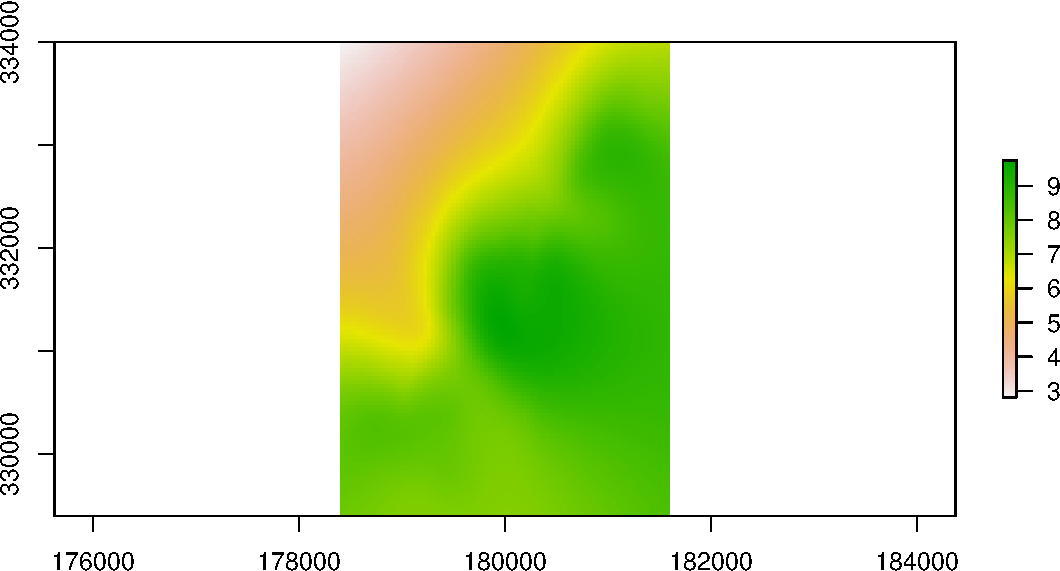
\includegraphics[width=0.95\textwidth]{Lec17_files/figure-beamer/unnamed-chunk-40-1} \end{center}

\end{frame}

\begin{frame}[fragile]{Hacky Crap}

\begin{Shaded}
\begin{Highlighting}[]
\NormalTok{p =}\StringTok{ }\KeywordTok{rasterToPolygons}\NormalTok{(meuse_elev_pred) }\OperatorTok\StringTok{ }\KeywordTok{st_as_sf}\NormalTok{()}
\KeywordTok{grid.arrange}\NormalTok{(}
  \KeywordTok{ggplot}\NormalTok{() }\OperatorTok{+}\StringTok{ }\KeywordTok{geom_sf}\NormalTok{(}\DataTypeTok{data=}\NormalTok{meuse, }\KeywordTok{aes}\NormalTok{(}\DataTypeTok{color=}\NormalTok{elev), }\DataTypeTok{size=}\FloatTok{0.1}\NormalTok{),}
  \KeywordTok{ggplot}\NormalTok{() }\OperatorTok{+}\StringTok{ }\KeywordTok{geom_sf}\NormalTok{(}\DataTypeTok{data=}\NormalTok{p, }\KeywordTok{aes}\NormalTok{(}\DataTypeTok{fill=}\NormalTok{test), }\DataTypeTok{color=}\OtherTok{NA}\NormalTok{),}
  \DataTypeTok{ncol=}\DecValTok{2}
\NormalTok{)}
\end{Highlighting}
\end{Shaded}

\begin{center}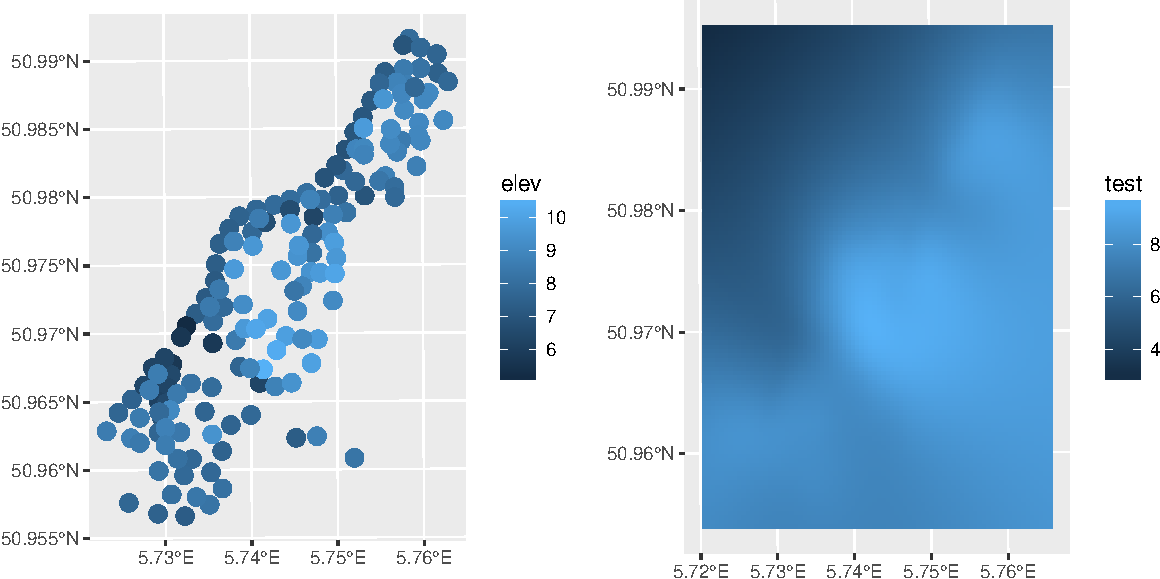
\includegraphics[width=0.95\textwidth]{Lec17_files/figure-beamer/unnamed-chunk-41-1} \end{center}

\end{frame}

\end{document}
